\documentclass[11pt,a4paper]{article}

% ============================================================
% Idioma, codificación y tipografía
% ============================================================
\usepackage[T1]{fontenc}
\usepackage[utf8]{inputenc}
\usepackage[spanish,es-nodecimaldot]{babel}
\usepackage{lmodern}
\usepackage{microtype}
\usepackage{csquotes}

\addto\captionsspanish{
    \renewcommand{\tablename}{Tabla}
    \renewcommand{\refname}{Referencias}
}

% ============================================================
% Configuración de página
% ============================================================
\usepackage[
    top=2.35cm,
    bottom=2.35cm,
    left=2.55cm,
    right=2.55cm
]{geometry}

\usepackage{setspace}
\setstretch{1.06}

\setlength{\parindent}{0pt}
\setlength{\parskip}{0.52em}

% ============================================================
% Matemática
% ============================================================
\usepackage{amsmath}
\usepackage{amssymb}
\usepackage{mathtools}

\newcommand{\Nact}[2]{N_{\mathrm{act}}^{\min}(#1,#2)}
\newcommand{\DeltaA}{\Delta A}
\newcommand{\DeltaB}{\Delta B}
\newcommand{\GF}{\mathrm{GF}(2)}

% ============================================================
% Tablas, figuras y control de saltos
% ============================================================
\usepackage{booktabs}
\usepackage{array}
\usepackage{tabularx}
\usepackage{graphicx}
\usepackage{float}
\usepackage{caption}
\usepackage{needspace}

\captionsetup{
    font=small,
    labelfont=bf,
    justification=centering
}

% ============================================================
% Listas
% ============================================================
\usepackage{enumitem}

\setlist[itemize]{
    leftmargin=1.45em,
    itemsep=0.20em,
    topsep=0.25em
}

\setlist[enumerate]{
    leftmargin=1.65em,
    itemsep=0.20em,
    topsep=0.25em
}

% ============================================================
% Colores y bloques de código
% ============================================================
\usepackage{xcolor}
\usepackage{listings}

\definecolor{grisclaro}{RGB}{246,246,246}
\definecolor{grisborde}{RGB}{190,190,190}

\lstset{
    basicstyle=\ttfamily\small,
    backgroundcolor=\color{grisclaro},
    frame=single,
    rulecolor=\color{grisborde},
    breaklines=true,
    showstringspaces=false,
    columns=fullflexible,
    keepspaces=true,
    xleftmargin=0.4em,
    xrightmargin=0.4em,
    aboveskip=0.7em,
    belowskip=0.7em
}

% ============================================================
% Diagramas
% ============================================================
\usepackage{tikz}
\usetikzlibrary{
    positioning,
    arrows.meta,
    shapes.geometric
}

% ============================================================
% Enlaces y metadatos
% ============================================================
\usepackage[hidelinks]{hyperref}
\urlstyle{same}

\hypersetup{
    pdftitle={
        Modelado MILP de Keccak reducido para la minimización
        de S-boxes activas
    },
    pdfauthor={Henry Sánchez Alvarado},
    pdfsubject={
        Criptoanálisis, Programación Lineal Entera Mixta y Keccak
    },
    pdfkeywords={
        Keccak, MILP, CBC, PuLP, S-boxes activas, criptoanálisis
    }
}

% ============================================================
% Bibliografía
% ============================================================
\usepackage[
    backend=biber,
    style=numeric,
    sorting=none,
    giveninits=true,
    maxbibnames=20
]{biblatex}

\addbibresource{references.bib}

% ============================================================
% Datos del artículo
% ============================================================
\title{
    \textbf{
        Modelado MILP de Keccak reducido para la minimización
        de S-boxes activas
    }
}

\author{
    Henry Sánchez Alvarado\\[0.35em]
    \small MCC640B Tópicos Especiales IV:
    Criptoanálisis, Codificación y Seguridad\\
    \small Profesor: Manuel Alejandro Quispe Torres\\
    \small Maestría en Ciencias de la Computación\\
    \small Universidad Nacional de Ingeniería
}

\date{Julio de 2026}

% ============================================================
% Documento
% ============================================================
\begin{document}

\maketitle

\begin{abstract}
Este trabajo presenta un modelo de Programación Lineal Entera Mixta
(MILP) para estudiar el número mínimo de aplicaciones activas de la
capa no lineal $\chi$ en versiones reducidas de Keccak. La formulación
representa bit a bit dos ejecuciones de la permutación y calcula sus
diferencias mediante restricciones XOR exactas. Se analizan tamaños de
palabra $z=4$ y $z=8$, correspondientes a estados de 100 y 200 bits y
a 20 y 40 aplicaciones locales de $\chi$ por ronda, respectivamente.

El modelo se implementó en Python con PuLP y se resolvió mediante CBC.
Para una ronda se certificó un mínimo global de una S-box activa, mientras
que para dos rondas se demostró un mínimo global de cuatro, con distribución
$2+2$. Para tres rondas se obtuvo la cota inferior global de cinco y se
construyeron testigos con actividades $2+2+9$ para $z=4$ y $2+2+10$
para $z=8$. Estos últimos valores son óptimos dentro de la familia
restringida $2+2+c$ y establecen las cotas superiores globales 13 y 14,
pero no mínimos globales de tres rondas.

Los resultados se validaron mediante una implementación funcional
independiente, reconstrucción de testigos y pruebas automatizadas.
\end{abstract}

\noindent\textbf{Palabras clave:} Keccak, programación lineal entera mixta,
criptoanálisis diferencial, S-boxes activas, PuLP, CBC.

% ============================================================
% Secciones
% ============================================================
\section{Introducción}
\label{sec:introduccion}

El análisis diferencial estudia cómo las diferencias entre dos entradas se
propagan a través de una primitiva criptográfica. Dentro de este enfoque, el
número de componentes no lineales activados constituye un indicador
estructural relevante: cuanto mayor sea la cantidad de componentes activos,
mayor será la dispersión de la diferencia y, en general, más difícil resultará
construir trayectorias diferenciales de baja complejidad
\cite{biham1991differential}.

Keccak, base del estándar SHA-3, organiza su estado como un arreglo
tridimensional de bits y aplica en cada ronda las transformaciones
$\theta$, $\rho$, $\pi$, $\chi$ e $\iota$
\cite{nist_fips202,bertoni2011keccak_reference}. Las transformaciones $\theta$, $\rho$
y $\pi$ producen difusión y reorganización del estado, mientras que $\chi$
constituye la única capa no lineal de la ronda. La transformación $\iota$
incorpora una constante dependiente del número de ronda.

La capa $\chi$ opera localmente sobre grupos de cinco bits que comparten las
mismas coordenadas $(y,k)$. En este trabajo, cada uno de estos grupos se
interpreta como una S-box local de cinco bits. Una S-box se considera activa
cuando al menos uno de sus bits de entrada presenta una diferencia no nula
entre dos ejecuciones de Keccak.

Determinar manualmente el número mínimo de S-boxes activas resulta difícil
incluso para versiones reducidas de la permutación. Las diferencias son
reorganizadas por las transformaciones lineales y posteriormente atraviesan
la capa no lineal, lo que produce un espacio combinatorio que crece con el
tamaño del estado y con el número de rondas.

La Programación Lineal Entera Mixta
(\emph{Mixed-Integer Linear Programming}, MILP) permite representar este
problema mediante variables binarias, restricciones lineales y una función
objetivo. Esta metodología ha sido utilizada para automatizar la búsqueda de
características diferenciales y lineales en distintas primitivas
criptográficas \cite{mouha2012milp,sun2014automatic}.

El presente trabajo desarrolla un modelo MILP bit a bit para versiones
reducidas de Keccak con tamaños de palabra

\[
z \in \{4,8\}.
\]

Estas configuraciones producen estados de

\[
25z
\]

bits; por tanto, se estudian estados de 100 bits para $z=4$ y de 200 bits
para $z=8$. Debido a que existen cinco valores posibles de $y$ y $z$
posiciones dentro de cada palabra, cada ronda contiene

\[
5z
\]

aplicaciones locales de $\chi$. En consecuencia, los experimentos consideran
20 S-boxes por ronda para $z=4$ y 40 S-boxes por ronda para $z=8$.

El modelo representa simultáneamente dos ejecuciones concretas de Keccak.
Las diferencias se calculan mediante restricciones XOR exactas, en lugar de
utilizar una aproximación diferencial truncada de la capa $\chi$. Esta
decisión permite reconstruir parejas concretas de estados, verificar la
propagación bit a bit y validar independientemente los patrones de actividad
obtenidos.

La implementación se desarrolló en Python utilizando PuLP como biblioteca
de modelado y CBC como solver de programación entera. El análisis comprende
una, dos y tres rondas de Keccak reducido.


\subsection{Planteamiento del problema}
\label{subsec:planteamiento}

Sean $A_0^L$ y $A_0^R$ dos estados iniciales distintos de Keccak reducido.
Su diferencia inicial se define como

\[
\Delta A_0 = A_0^L \oplus A_0^R,
\]

con la condición

\[
\Delta A_0 \neq 0.
\]

Durante cada ronda, ambos estados atraviesan las transformaciones

\[
\theta \longrightarrow \rho \longrightarrow \pi
\longrightarrow \chi \longrightarrow \iota.
\]

Sea $\Delta B_r$ la diferencia entre las dos ejecuciones inmediatamente
antes de la capa $\chi$ en la ronda $r$. Una aplicación local de $\chi$,
identificada por las coordenadas $(y,k)$, se considera activa cuando

\[
\bigvee_{x=0}^{4} \Delta B_r[x,y,k] = 1.
\]

El problema consiste en minimizar la suma de S-boxes activas durante $R$
rondas, bajo la condición de que los estados iniciales sean diferentes.

La pregunta central del trabajo es la siguiente:

\begin{quote}
¿Cuál es el número mínimo de aplicaciones activas de la capa $\chi$ que
puede presentar una diferencia inicial no nula al propagarse durante una,
dos y tres rondas de Keccak reducido para $z=4$ y $z=8$?
\end{quote}

El número mínimo de S-boxes activas se denota por

\[
N_{\mathrm{act}}^{\min}(z,R),
\]

donde $z$ es el tamaño de palabra y $R$ es el número de rondas analizadas.

Para una y dos rondas se busca establecer mínimos globales mediante la
coincidencia entre una cota inferior demostrada y un testigo factible. Para
tres rondas, debido al crecimiento del espacio combinatorio, se busca
establecer cotas globales y construir testigos verificables mediante una
búsqueda exhaustiva restringida.


\subsection{Correspondencia experimental entre intentos y rondas}
\label{subsec:intentos_rondas}

La actividad académica propone relacionar tres rangos de intentos con
experimentos de una, dos y tres rondas. En este trabajo se adopta la
correspondencia

\[
R(t)=
\begin{cases}
1, & t < 10,\\
2, & 10 \leq t < 20,\\
3, & 20 \leq t < 30.
\end{cases}
\]

Esta relación se utiliza exclusivamente como criterio experimental para
seleccionar el número de rondas analizadas. El número de intentos no modifica
las transformaciones internas de Keccak y no representa una relación
criptográfica demostrada entre los intentos de un atacante y la profundidad
de la permutación.

Por esta razón, los resultados principales se expresan en términos del
tamaño de palabra $z$ y del número de rondas $R$.


\subsection{Objetivos}
\label{subsec:objetivos}

\subsubsection{Objetivo general}

Modelar una versión reducida de Keccak mediante Programación Lineal Entera
Mixta para determinar o acotar el número mínimo de S-boxes activas en una,
dos y tres rondas, utilizando CBC como solver.


\subsubsection{Objetivos específicos}

\begin{enumerate}
    \item Implementar las transformaciones $\theta$, $\rho$, $\pi$, $\chi$
    e $\iota$ para estados reducidos de Keccak con tamaños de palabra
    $z=4$ y $z=8$.

    \item Construir un modelo MILP bit a bit que represente dos ejecuciones
    simultáneas de Keccak y calcule exactamente sus diferencias mediante
    restricciones XOR.

    \item Definir variables binarias que identifiquen las aplicaciones
    activas de $\chi$ y formular una función objetivo que minimice su
    cantidad total.

    \item Analizar configuraciones de una, dos y tres rondas, distinguiendo
    entre mínimos globales, cotas inferiores, testigos factibles y óptimos
    restringidos.

    \item Validar los resultados mediante una implementación funcional
    independiente, reconstrucción de testigos y pruebas automatizadas.
\end{enumerate}


\subsection{Contribuciones}
\label{subsec:contribuciones}

Las principales contribuciones del trabajo son las siguientes:

\begin{enumerate}
    \item Una implementación funcional de las transformaciones
    $\theta$, $\rho$, $\pi$, $\chi$ e $\iota$ para versiones reducidas de
    Keccak.

    \item Una formulación MILP exacta que representa bit a bit dos
    ejecuciones de la permutación y calcula sus diferencias XOR.

    \item Un modelo de actividad que identifica cada aplicación local de
    $\chi$ activa y minimiza su suma durante varias rondas.

    \item La certificación de los mínimos globales

    \[
    N_{\mathrm{act}}^{\min}(4,1)
    =
    N_{\mathrm{act}}^{\min}(8,1)
    =
    1
    \]

    para una ronda, y

    \[
    N_{\mathrm{act}}^{\min}(4,2)
    =
    N_{\mathrm{act}}^{\min}(8,2)
    =
    4
    \]

    para dos rondas.

    \item La obtención de las cotas globales

    \[
    5
    \leq
    N_{\mathrm{act}}^{\min}(4,3)
    \leq
    13
    \]

    y

    \[
    5
    \leq
    N_{\mathrm{act}}^{\min}(8,3)
    \leq
    14
    \]

    para tres rondas.

    \item La construcción de testigos con distribuciones de actividad

    \[
    2+2+9
    \]

    para $z=4$ y

    \[
    2+2+10
    \]

    para $z=8$. Estos testigos son óptimos dentro de la familia restringida
    $2+2+c$ y proporcionan cotas superiores válidas para el problema
    global.

    \item Una estrategia de validación que contrasta las soluciones del
    modelo con una implementación funcional independiente y permite
    reconstruir los estados, las diferencias y los soportes activos.
\end{enumerate}


\subsection{Alcance}
\label{subsec:alcance}

El estudio se limita a versiones reducidas de Keccak con tamaños de palabra

\[
z \in \{4,8\}
\]

y a un máximo de tres rondas. Estas configuraciones conservan la estructura
de la permutación, pero no corresponden a la instancia completa
Keccak-$f[1600]$ utilizada por SHA-3.

La variable principal es el número de aplicaciones activas de la capa
$\chi$. Esta medida permite estudiar la propagación estructural de una
diferencia, pero no determina por sí sola la probabilidad de una
característica diferencial. El modelo no incorpora los pesos de las
transiciones diferenciales locales ni estima directamente la complejidad
de un ataque contra SHA-3.

Los resultados de una y dos rondas corresponden a mínimos globales
certificados. Para tres rondas, los valores 13 y 14 no se presentan como
mínimos globales. Estos valores son los mejores resultados obtenidos dentro
de la familia restringida

\[
2+2+c
\]

y deben interpretarse como cotas superiores globales respaldadas por
testigos concretos.

En consecuencia, el aporte del trabajo consiste en formular, resolver y
validar el problema de minimización de S-boxes activas para las
configuraciones reducidas consideradas, sin extender las conclusiones más
allá de las evidencias matemáticas y experimentales disponibles.
\section{Keccak reducido y modelo de actividad}
\label{sec:keccak_reducido}

Keccak es una familia de funciones criptográficas basada en una permutación
sobre un estado tridimensional de bits. El estándar SHA-3 utiliza
permutaciones de la familia Keccak-$p$ y define cada ronda mediante la
composición de cinco transformaciones:

\[
\theta
\longrightarrow
\rho
\longrightarrow
\pi
\longrightarrow
\chi
\longrightarrow
\iota.
\]

Las transformaciones $\theta$, $\rho$ y $\pi$ conforman la parte lineal de
la ronda. La transformación $\chi$ introduce la no linealidad, mientras que
$\iota$ incorpora una constante dependiente del número de ronda
\cite{nist_fips202,bertoni2011keccak_reference}.

En este trabajo se conserva la estructura de la ronda de Keccak, pero se
emplean tamaños de palabra reducidos para hacer viable la construcción y
resolución del modelo MILP.


\subsection{Representación del estado}
\label{subsec:representacion_estado}

El estado al inicio de la ronda $r$ se representa mediante el arreglo
binario

\[
A_r[x,y,k] \in \{0,1\},
\]

donde

\[
x,y \in \{0,1,2,3,4\},
\qquad
k \in \{0,\ldots,z-1\}.
\]

Las coordenadas $(x,y)$ identifican una de las 25 palabras o
\emph{lanes} del estado, mientras que $k$ identifica una posición dentro
de una palabra de longitud $z$. Por tanto, el tamaño total del estado es

\[
25z \text{ bits}.
\]

Se analizan los tamaños de palabra $z=4$ y $z=8$. La
Tabla~\ref{tab:configuraciones_keccak} resume las configuraciones
consideradas.

\begin{table}[htbp]
    \centering
    \caption{Configuraciones reducidas de Keccak consideradas en el trabajo.}
    \label{tab:configuraciones_keccak}
    \begin{tabular}{cccc}
        \hline
        $z$ & Tamaño del estado & Palabras & S-boxes por ronda \\
        \hline
        4 & 100 bits & 25 & 20 \\
        8 & 200 bits & 25 & 40 \\
        \hline
    \end{tabular}
\end{table}

Cada aplicación local de $\chi$ procesa cinco bits que comparten las
coordenadas $(y,k)$ y recorren los cinco valores posibles de $x$. Como
existen cinco valores de $y$ y $z$ posiciones dentro de cada palabra, el
número de aplicaciones locales de $\chi$ por ronda es

\[
5z.
\]


\subsection{Transformaciones de una ronda}
\label{subsec:transformaciones_ronda}

Para distinguir los estados intermedios de una ronda se utiliza la siguiente
notación:

\[
T_r = \theta(A_r),
\]

\[
R_r = \rho(T_r),
\]

\[
B_r = \pi(R_r),
\]

\[
C_r = \chi(B_r),
\]

\[
A_{r+1} = \iota(C_r,r).
\]

El estado $B_r$ corresponde a la entrada de la capa no lineal $\chi$ y
será utilizado posteriormente para determinar qué S-boxes se encuentran
activas.


\subsubsection{Transformación \texorpdfstring{$\theta$}{theta}}

La transformación $\theta$ introduce difusión entre las columnas del
estado. Primero se calcula la paridad de cada columna:

\[
P_r[x,k]
=
\bigoplus_{y=0}^{4}
A_r[x,y,k].
\]

A partir de estas paridades se define el término de difusión

\[
D_r[x,k]
=
P_r[(x-1)\bmod 5,k]
\oplus
P_r[(x+1)\bmod 5,(k-1)\bmod z].
\]

La salida de $\theta$ es

\[
T_r[x,y,k]
=
A_r[x,y,k]
\oplus
D_r[x,k].
\]

La transformación $\theta$ es lineal sobre $\mathrm{GF}(2)$ y distribuye
la información de la paridad de una columna hacia columnas vecinas.


\subsubsection{Transformaciones \texorpdfstring{$\rho$}{rho} y
\texorpdfstring{$\pi$}{pi}}

La transformación $\rho$ rota cada palabra según un desplazamiento
predefinido. Los desplazamientos especificados por Keccak se interpretan
módulo $z$:

\[
R_r[x,y,k]
=
T_r
\left[
x,
y,
\bigl(k-r[x,y]\bigr)\bmod z
\right],
\]

donde $r[x,y]$ representa el desplazamiento asignado a la palabra
$(x,y)$.

La transformación $\pi$ reorganiza las palabras dentro del estado:

\[
B_r
\left[
y,
(2x+3y)\bmod 5,
k
\right]
=
R_r[x,y,k].
\]

Las transformaciones $\rho$ y $\pi$ son permutaciones de posiciones. Por
tanto, no modifican los valores de los bits, sino únicamente su ubicación
dentro del estado.


\subsubsection{Transformación \texorpdfstring{$\chi$}{chi}}

La transformación $\chi$ constituye la única capa no lineal de la ronda.
Para cada posición $(y,k)$ opera sobre los cinco bits obtenidos al variar
$x$:

\[
C_r[x,y,k]
=
B_r[x,y,k]
\oplus
\left[
\left(
1 \oplus B_r[(x+1)\bmod 5,y,k]
\right)
B_r[(x+2)\bmod 5,y,k]
\right].
\]

Cada conjunto

\[
\left(
B_r[0,y,k],
B_r[1,y,k],
B_r[2,y,k],
B_r[3,y,k],
B_r[4,y,k]
\right)
\]

se interpreta en este trabajo como una S-box local de cinco bits.

Esta denominación no implica que Keccak utilice una tabla de sustitución
independiente en el sentido tradicional. Se emplea porque cada grupo local
de cinco bits constituye una unidad no lineal cuya actividad puede
contabilizarse durante la propagación diferencial.


\subsubsection{Transformación \texorpdfstring{$\iota$}{iota}}

La transformación $\iota$ incorpora una constante de ronda en la palabra
ubicada en las coordenadas $(0,0)$. Su acción puede expresarse como

\[
A_{r+1}[x,y,k]
=
\begin{cases}
C_r[0,0,k] \oplus RC_r[k],
    & \text{si } (x,y)=(0,0),\\[4pt]
C_r[x,y,k],
    & \text{en otro caso},
\end{cases}
\]

donde $RC_r[k]$ representa el bit correspondiente de la constante de la
ronda $r$.

Para los tamaños de palabra $z=4$ y $z=8$, las constantes se restringen a
las primeras $z$ posiciones de la palabra.


\subsection{Modelo diferencial pareado}
\label{subsec:modelo_diferencial_pareado}

El análisis considera dos ejecuciones simultáneas de Keccak, denominadas
ejecución izquierda y ejecución derecha. Sus estados al inicio de la ronda
$r$ se representan mediante

\[
A_r^L
\qquad \text{y} \qquad
A_r^R.
\]

La diferencia entre ambos estados se define mediante XOR:

\[
\Delta A_r
=
A_r^L \oplus A_r^R.
\]

De forma análoga, los estados inmediatamente anteriores a la capa $\chi$
son

\[
B_r^L
=
(\pi \circ \rho \circ \theta)(A_r^L),
\]

\[
B_r^R
=
(\pi \circ \rho \circ \theta)(A_r^R),
\]

y su diferencia es

\[
\Delta B_r
=
B_r^L \oplus B_r^R.
\]

La utilización de dos ejecuciones concretas permite representar
exactamente el comportamiento de la capa no lineal. En lugar de aproximar
la propagación diferencial de $\chi$, se evalúa la transformación sobre
ambos estados y posteriormente se calcula la diferencia entre sus salidas.

La constante de ronda aplicada por $\iota$ es idéntica en las dos
ejecuciones. En consecuencia, se cancela al calcular la diferencia:

\[
\left(
C_r^L \oplus RC_r
\right)
\oplus
\left(
C_r^R \oplus RC_r
\right)
=
C_r^L \oplus C_r^R.
\]

Aunque $\iota$ no modifica la diferencia, se conserva en la implementación
para mantener una representación exacta de los estados absolutos y permitir
la reconstrucción completa de los testigos.


\subsection{Definición de S-box activa}
\label{subsec:sbox_activa}

Una aplicación local de $\chi$ en la posición $(y,k)$ de la ronda $r$ se
considera activa cuando al menos uno de sus cinco bits de entrada presenta
una diferencia no nula.

Se introduce el indicador binario

\[
a_{r,y,k} \in \{0,1\},
\]

definido por

\[
a_{r,y,k}
=
\bigvee_{x=0}^{4}
\Delta B_r[x,y,k].
\]

Por tanto,

\[
a_{r,y,k}=1
\]

si existe al menos un valor de $x$ para el cual

\[
\Delta B_r[x,y,k]=1.
\]

El número de S-boxes activas en la ronda $r$ se define como

\[
m_r
=
\sum_{y=0}^{4}
\sum_{k=0}^{z-1}
a_{r,y,k}.
\]

Para una ejecución de $R$ rondas, la actividad total es

\[
N_{\mathrm{act}}
=
\sum_{r=0}^{R-1}
m_r
=
\sum_{r=0}^{R-1}
\sum_{y=0}^{4}
\sum_{k=0}^{z-1}
a_{r,y,k}.
\]

El problema de optimización estudiado consiste en minimizar
$N_{\mathrm{act}}$ bajo la condición de que la diferencia inicial sea no
nula.


\subsection{Propiedades estructurales utilizadas}
\label{subsec:propiedades_estructurales}

La interpretación de los resultados utiliza las siguientes propiedades de
Keccak:

\begin{enumerate}
    \item Las transformaciones $\theta$, $\rho$ y $\pi$ son biyectivas.
    Por tanto, una diferencia no nula al inicio de una ronda no puede
    convertirse en una diferencia nula antes de alcanzar la capa $\chi$:

    \[
    \Delta A_r \neq 0
    \Longrightarrow
    \Delta B_r \neq 0.
    \]

    \item La ronda completa de Keccak es una permutación. En consecuencia,
    dos estados distintos continúan siendo distintos después de aplicar
    cualquier número de rondas:

    \[
    A_r^L \neq A_r^R
    \Longrightarrow
    A_{r+1}^L \neq A_{r+1}^R.
    \]

    \item La transformación $\iota$ no modifica la diferencia entre las
    dos ejecuciones porque aplica la misma constante a ambas.

    \item Una diferencia no nula en $B_r$ activa necesariamente al menos
    una aplicación local de $\chi$:

    \[
    \Delta B_r \neq 0
    \Longrightarrow
    m_r \geq 1.
    \]
\end{enumerate}

Estas propiedades permiten establecer cotas inferiores básicas para una o
varias rondas. La forma en que se incorporan al modelo MILP y se utilizan
para certificar los resultados se desarrolla en las secciones siguientes.
\section{Formulación MILP}
\label{sec:formulacion_milp}

El problema de minimizar el número de S-boxes activas se formula mediante
Programación Lineal Entera Mixta. El modelo representa bit a bit dos
ejecuciones de Keccak reducido, denominadas izquierda y derecha, e impone
de manera exacta las transformaciones de cada ronda.

A diferencia de una formulación diferencial truncada, el modelo conserva
los valores absolutos de ambos estados. Las diferencias se calculan mediante
restricciones XOR y la propagación a través de $\chi$ se obtiene evaluando
la función booleana en las dos ejecuciones.

Esta representación incrementa el número de variables, pero permite
reconstruir parejas concretas de estados y verificar independientemente
las soluciones obtenidas por el solver.


\subsection{Índices y variables}
\label{subsec:variables_milp}

Los índices utilizados son

\[
r \in \{0,\ldots,R-1\},
\qquad
x,y \in \{0,\ldots,4\},
\qquad
k \in \{0,\ldots,z-1\},
\]

donde $r$ identifica la ronda, $(x,y)$ identifica una palabra del estado
y $k$ representa una posición dentro de la palabra.

Las dos ejecuciones se identifican mediante

\[
\sigma \in \{L,R\}.
\]

Para cada ejecución se introducen las variables binarias

\[
A_{r,x,y,k}^{\sigma} \in \{0,1\},
\]

que representan el estado al inicio de la ronda $r$.

Los estados intermedios se representan mediante

\[
T_{r,x,y,k}^{\sigma},
\qquad
R_{r,x,y,k}^{\sigma},
\qquad
B_{r,x,y,k}^{\sigma},
\qquad
C_{r,x,y,k}^{\sigma},
\]

donde:

\begin{itemize}
    \item $T^\sigma_r$ es la salida de $\theta$;
    \item $R^\sigma_r$ es la salida de $\rho$;
    \item $B^\sigma_r$ es la salida de $\pi$ y la entrada de $\chi$;
    \item $C^\sigma_r$ es la salida de $\chi$.
\end{itemize}

También se introducen variables de diferencia

\[
\Delta A_{r,x,y,k} \in \{0,1\},
\qquad
\Delta B_{r,x,y,k} \in \{0,1\},
\]

y variables de actividad

\[
a_{r,y,k} \in \{0,1\}.
\]


\subsection{Linealización de la operación XOR}
\label{subsec:xor_milp}

Sean $u$, $v$ y $d$ variables binarias relacionadas mediante

\[
d = u \oplus v.
\]

La operación XOR se representa exactamente introduciendo una variable
auxiliar binaria $q$ y la igualdad

\[
u+v=d+2q.
\label{eq:xor_lineal}
\]

Esta restricción reproduce las cuatro combinaciones posibles:

\[
\begin{array}{c|c|c}
u & v & d\\
\hline
0 & 0 & 0\\
0 & 1 & 1\\
1 & 0 & 1\\
1 & 1 & 0
\end{array}
\]

La misma construcción se utiliza en todas las operaciones XOR binarias
del modelo. Cuando es necesario calcular el XOR de más de dos bits, la
operación se descompone en una secuencia de XOR binarios.

Las diferencias entre las dos ejecuciones se definen mediante

\[
\Delta A_{r,x,y,k}
=
A_{r,x,y,k}^{L}
\oplus
A_{r,x,y,k}^{R},
\]

y

\[
\Delta B_{r,x,y,k}
=
B_{r,x,y,k}^{L}
\oplus
B_{r,x,y,k}^{R}.
\]


\subsection{Representación de las capas lineales}
\label{subsec:capas_lineales_milp}

Las transformaciones $\theta$, $\rho$ y $\pi$ se incorporan de manera
independiente para cada ejecución $\sigma$.


\subsubsection{Transformación \texorpdfstring{$\theta$}{theta}}

Para cada columna se calcula la paridad

\[
P_{r,x,k}^{\sigma}
=
\bigoplus_{y=0}^{4}
A_{r,x,y,k}^{\sigma}.
\]

En la implementación, este XOR de cinco bits se construye mediante
operaciones XOR binarias sucesivas.

El término de difusión se define como

\[
D_{r,x,k}^{\sigma}
=
P_{r,(x-1)\bmod 5,k}^{\sigma}
\oplus
P_{r,(x+1)\bmod 5,(k-1)\bmod z}^{\sigma}.
\]

La salida de $\theta$ satisface

\[
T_{r,x,y,k}^{\sigma}
=
A_{r,x,y,k}^{\sigma}
\oplus
D_{r,x,k}^{\sigma}.
\]

Todas estas relaciones se linealizan utilizando la
Ecuación~\ref{eq:xor_lineal}.


\subsubsection{Transformaciones \texorpdfstring{$\rho$}{rho} y
\texorpdfstring{$\pi$}{pi}}

Las transformaciones $\rho$ y $\pi$ son permutaciones de bits. Por tanto,
se representan mediante igualdades directas y no requieren variables
auxiliares de producto.

La transformación $\rho$ se impone mediante

\[
R_{r,x,y,k}^{\sigma}
=
T_{r,x,y,(k-r[x,y])\bmod z}^{\sigma}.
\]

La transformación $\pi$ se representa como

\[
B_{r,y,(2x+3y)\bmod 5,k}^{\sigma}
=
R_{r,x,y,k}^{\sigma}.
\]

Estas restricciones conservan el valor de cada bit y modifican únicamente
su posición dentro del estado.


\subsection{Representación exacta de la capa \texorpdfstring{$\chi$}{chi}}
\label{subsec:chi_milp}

Para cada ejecución $\sigma$, la transformación $\chi$ se define por

\[
C_{r,x,y,k}^{\sigma}
=
B_{r,x,y,k}^{\sigma}
\oplus
\left[
\left(
1-B_{r,(x+1)\bmod 5,y,k}^{\sigma}
\right)
B_{r,(x+2)\bmod 5,y,k}^{\sigma}
\right].
\]

La expresión contiene el producto de dos variables binarias. Para
linealizarlo se introduce

\[
s_{r,x,y,k}^{\sigma} \in \{0,1\},
\]

con

\[
s_{r,x,y,k}^{\sigma}
=
\left(
1-B_{r,(x+1)\bmod 5,y,k}^{\sigma}
\right)
B_{r,(x+2)\bmod 5,y,k}^{\sigma}.
\]

La conjunción se representa mediante las restricciones

\[
s_{r,x,y,k}^{\sigma}
\leq
1-B_{r,(x+1)\bmod 5,y,k}^{\sigma},
\]

\[
s_{r,x,y,k}^{\sigma}
\leq
B_{r,(x+2)\bmod 5,y,k}^{\sigma},
\]

\[
s_{r,x,y,k}^{\sigma}
\geq
B_{r,(x+2)\bmod 5,y,k}^{\sigma}
-
B_{r,(x+1)\bmod 5,y,k}^{\sigma}.
\]

Como todas las variables son binarias, estas desigualdades fuerzan
exactamente el valor del producto.

La salida de $\chi$ se obtiene mediante

\[
C_{r,x,y,k}^{\sigma}
=
B_{r,x,y,k}^{\sigma}
\oplus
s_{r,x,y,k}^{\sigma},
\]

que se linealiza nuevamente mediante la
Ecuación~\ref{eq:xor_lineal}.

La formulación se aplica por separado a las ejecuciones izquierda y
derecha. La diferencia de salida surge, por tanto, de dos evaluaciones
exactas de la función booleana $\chi$.


\subsection{Representación de la capa \texorpdfstring{$\iota$}{iota}}
\label{subsec:iota_milp}

La constante de ronda es conocida y no constituye una variable de decisión.

Para la palabra $(0,0)$, si el bit correspondiente de la constante es cero,
se impone

\[
A_{r+1,0,0,k}^{\sigma}
=
C_{r,0,0,k}^{\sigma}.
\]

Si el bit de la constante es uno, se utiliza

\[
A_{r+1,0,0,k}^{\sigma}
=
1-C_{r,0,0,k}^{\sigma}.
\]

Para las demás posiciones se imponen igualdades directas:

\[
A_{r+1,x,y,k}^{\sigma}
=
C_{r,x,y,k}^{\sigma},
\qquad
(x,y)\neq(0,0).
\]

Aunque la misma constante se cancela al calcular la diferencia entre
ejecuciones, su inclusión permite representar y reconstruir correctamente
los estados absolutos.


\subsection{Variables de actividad}
\label{subsec:variables_actividad_milp}

La variable

\[
a_{r,y,k} \in \{0,1\}
\]

indica si la aplicación local de $\chi$ situada en $(y,k)$ se encuentra
activa durante la ronda $r$.

Esta variable debe valer uno cuando al menos uno de los cinco bits de
entrada presenta una diferencia no nula. La relación OR se representa
mediante

\[
a_{r,y,k}
\geq
\Delta B_{r,x,y,k},
\qquad
x\in\{0,\ldots,4\},
\]

y

\[
a_{r,y,k}
\leq
\sum_{x=0}^{4}
\Delta B_{r,x,y,k}.
\]

Si los cinco bits de diferencia son cero, la segunda restricción fuerza

\[
a_{r,y,k}=0.
\]

Si al menos uno de los bits es uno, alguna de las cotas inferiores fuerza

\[
a_{r,y,k}=1.
\]

El número de S-boxes activas en la ronda $r$ es

\[
m_r
=
\sum_{y=0}^{4}
\sum_{k=0}^{z-1}
a_{r,y,k}.
\]


\subsection{Condición de diferencia inicial no nula}
\label{subsec:diferencia_inicial_milp}

Sin una restricción adicional, el modelo admitiría como solución trivial
dos estados iniciales idénticos, cuya actividad total sería cero.

Para excluir esta solución se impone

\[
\sum_{x=0}^{4}
\sum_{y=0}^{4}
\sum_{k=0}^{z-1}
\Delta A_{0,x,y,k}
\geq
1.
\]

Esta condición garantiza que

\[
A_0^L \neq A_0^R.
\]


\subsection{Función objetivo}
\label{subsec:funcion_objetivo_milp}

La actividad total durante $R$ rondas se define como

\[
N_{\mathrm{act}}
=
\sum_{r=0}^{R-1}
\sum_{y=0}^{4}
\sum_{k=0}^{z-1}
a_{r,y,k}.
\]

La función objetivo es

\[
\min
\sum_{r=0}^{R-1}
\sum_{y=0}^{4}
\sum_{k=0}^{z-1}
a_{r,y,k}.
\label{eq:funcion_objetivo}
\]

Cuando el solver demuestra la optimalidad global, el valor de la
Ecuación~\ref{eq:funcion_objetivo} corresponde a

\[
N_{\mathrm{act}}^{\min}(z,R).
\]

Cuando se obtiene únicamente una solución factible, su actividad constituye
una cota superior para el mínimo global.


\subsection{Restricciones auxiliares}
\label{subsec:restricciones_auxiliares}

Además del problema de minimización, la implementación permite incorporar
restricciones auxiliares para certificar cotas y validar testigos.


\subsubsection{Cota sobre la actividad total}

Para comprobar si existe una trayectoria con actividad no mayor que un
valor $U$, se añade

\[
N_{\mathrm{act}} \leq U.
\]

Si el solver demuestra que este problema es infactible, se concluye que no
existe una trayectoria válida con actividad total menor o igual que $U$.


\subsubsection{Actividad exacta por ronda}

El número de S-boxes activas en una ronda concreta puede fijarse mediante

\[
m_r
=
\sum_{y=0}^{4}
\sum_{k=0}^{z-1}
a_{r,y,k}
=
\widehat{m}_r,
\]

donde $\widehat{m}_r$ es el valor impuesto.

Esta restricción permite estudiar distribuciones como

\[
2+2
\]

o

\[
2+2+c.
\]


\subsubsection{Fijación de soportes activos}

Sea

\[
S_r
\subseteq
\{0,\ldots,4\}
\times
\{0,\ldots,z-1\}
\]

un soporte activo conocido. Puede imponerse

\[
a_{r,y,k}=1
\qquad
\text{si }(y,k)\in S_r,
\]

y

\[
a_{r,y,k}=0
\qquad
\text{si }(y,k)\notin S_r.
\]

Esta operación se utiliza para comprobar con el modelo MILP los soportes
obtenidos mediante búsqueda o reconstrucción.


\subsubsection{Fijación de estados concretos}

Los estados iniciales de un testigo pueden fijarse mediante

\[
A_{0,x,y,k}^{L}
=
\widehat{A}_{0,x,y,k}^{L},
\]

\[
A_{0,x,y,k}^{R}
=
\widehat{A}_{0,x,y,k}^{R}.
\]

Con ambos estados fijados, el modelo verifica que las transformaciones, las
diferencias y la actividad reportada sean consistentes con todas las
restricciones.


\subsection{Interpretación de los resultados del solver}
\label{subsec:interpretacion_solver}

La interpretación del resultado depende del estado de terminación del
solver:

\begin{description}
    \item[Óptimo global.] Se encontró una solución factible y se demostró
    que no existe otra con menor valor objetivo.

    \item[Solución factible.] Se encontró un testigo válido, pero no se
    demostró la optimalidad. Su valor constituye una cota superior.

    \item[Infactible.] Se demostró que ninguna solución satisface las
    restricciones impuestas. Este resultado puede utilizarse para elevar
    una cota inferior.

    \item[Límite de tiempo.] La terminación por tiempo no demuestra por sí
    sola optimalidad, infactibilidad ni ausencia de soluciones.
\end{description}

Esta distinción es fundamental en los experimentos de tres rondas. Los
testigos con actividades 13 y 14 demuestran cotas superiores globales,
pero su optimalidad solo fue establecida dentro de la familia restringida

\[
2+2+c.
\]
\section{Arquitectura e implementación}
\label{sec:arquitectura_implementacion}

La implementación se desarrolló en Python siguiendo una arquitectura
modular que separa la especificación funcional de Keccak, la formulación
MILP, la búsqueda de trayectorias, la validación de testigos y la
generación de resultados.

Esta separación permite contrastar las soluciones del solver con una
implementación que no depende del modelo de optimización. De este modo,
el valor objetivo informado por CBC no se acepta de manera aislada, sino
que se verifica mediante la reconstrucción completa de los estados y de
sus diferencias.

PuLP se utilizó como biblioteca de modelado y CBC como solver de
programación lineal entera mixta
\cite{pulp_docs,cbc_guide}.


\subsection{Arquitectura general}
\label{subsec:arquitectura_general}

El flujo de trabajo se organiza en cinco etapas:

\begin{enumerate}
    \item implementar las transformaciones de Keccak reducido mediante
    funciones binarias de referencia;

    \item construir el modelo MILP exacto para dos ejecuciones simultáneas;

    \item incorporar las diferencias XOR, las variables de actividad y la
    función objetivo;

    \item resolver los experimentos mediante CBC o mediante una búsqueda
    restringida para tres rondas;

    \item reconstruir y validar los testigos con la implementación
    funcional independiente.
\end{enumerate}

El flujo puede resumirse como

\[
\text{Keccak de referencia}
\longrightarrow
\text{modelo MILP pareado}
\longrightarrow
\text{búsqueda de soluciones}
\longrightarrow
\text{reconstrucción}
\longrightarrow
\text{validación}.
\]

La arquitectura distingue claramente entre la obtención de una solución
y su comprobación. Esto reduce el riesgo de aceptar resultados producidos
por errores en la formulación, en la extracción de variables o en la
interpretación del estado del solver.


\subsection{Componentes principales}
\label{subsec:componentes_principales}

La Tabla~\ref{tab:componentes_implementacion} resume los componentes
principales del proyecto.

\begin{table}[htbp]
    \centering
    \caption{Componentes principales de la implementación.}
    \label{tab:componentes_implementacion}
    \begin{tabular}{p{0.31\textwidth}p{0.61\textwidth}}
        \hline
        \textbf{Componente} & \textbf{Responsabilidad} \\
        \hline

        Implementación de referencia
        &
        Ejecuta las transformaciones $\theta$, $\rho$, $\pi$, $\chi$ e
        $\iota$ directamente sobre arreglos binarios.
        \\[3pt]

        Modelo MILP de Keccak
        &
        Representa cada transformación mediante variables binarias,
        restricciones XOR, permutaciones y linealizaciones de productos.
        \\[3pt]

        Modelo diferencial pareado
        &
        Construye dos ejecuciones simultáneas y calcula las diferencias
        exactas en las fronteras de cada ronda.
        \\[3pt]

        Modelo de S-boxes activas
        &
        Incorpora las variables $a_{r,y,k}$, la función objetivo y las
        restricciones auxiliares para cotas, soportes y conteos por ronda.
        \\[3pt]

        Búsqueda restringida
        &
        Explora exhaustivamente trayectorias de tres rondas pertenecientes
        a la familia $2+2+c$.
        \\[3pt]

        Ejecutor experimental
        &
        Ejecuta los seis escenarios, almacena los resultados y genera los
        artefactos necesarios para su análisis.
        \\[3pt]

        Pruebas automatizadas
        &
        Verifican transformaciones, restricciones, testigos, búsquedas y
        archivos de salida.
        \\
        \hline
    \end{tabular}
\end{table}


\subsection{Implementación funcional de referencia}
\label{subsec:implementacion_referencia}

La implementación de referencia opera directamente sobre estados
binarios y reproduce el orden completo de una ronda:

\[
A_r
\xrightarrow{\theta}
T_r
\xrightarrow{\rho}
R_r
\xrightarrow{\pi}
B_r
\xrightarrow{\chi}
C_r
\xrightarrow{\iota}
A_{r+1}.
\]

Sus funciones se utilizan como una especificación independiente del
modelo MILP. En particular, permiten:

\begin{itemize}
    \item comprobar las transformaciones individuales;
    \item ejecutar una o varias rondas completas;
    \item reconstruir los estados obtenidos mediante el solver;
    \item recalcular las diferencias antes de cada aplicación de $\chi$;
    \item verificar el número de S-boxes activas por ronda.
\end{itemize}

La existencia de esta implementación independiente es importante porque
una solución MILP puede ser matemáticamente consistente con un modelo
incorrectamente programado. La comparación bit a bit permite detectar
este tipo de errores.


\subsection{Modelo MILP pareado}
\label{subsec:implementacion_modelo_pareado}

El modelo contiene dos copias de la permutación reducida:

\[
A_r^L
\qquad \text{y} \qquad
A_r^R.
\]

Cada ejecución satisface las restricciones exactas de las
transformaciones de Keccak. A partir de ambas copias se calculan las
diferencias

\[
\Delta A_r
=
A_r^L \oplus A_r^R,
\]

y

\[
\Delta B_r
=
B_r^L \oplus B_r^R.
\]

La clase que incorpora la minimización de actividad extiende este modelo
con las variables

\[
a_{r,y,k},
\]

que identifican las aplicaciones activas de $\chi$.

Además de la función objetivo global, la implementación permite:

\begin{itemize}
    \item imponer una cota sobre la actividad total;
    \item fijar el número de S-boxes activas en una ronda;
    \item fijar un soporte activo concreto;
    \item fijar los estados iniciales izquierdo y derecho;
    \item extraer los estados y soportes de una solución.
\end{itemize}

Estas operaciones se utilizan tanto para resolver los problemas de
optimización como para validar candidatos generados por otros
procedimientos.


\subsection{Búsqueda restringida para tres rondas}
\label{subsec:busqueda_restringida_implementacion}

La resolución directa del modelo global de tres rondas presenta un
crecimiento considerable del espacio combinatorio. Para obtener testigos
reproducibles se implementó una búsqueda restringida a trayectorias con
actividad

\[
2+2+c.
\]

La elección de esta familia parte del resultado exacto de dos rondas:
existen trayectorias globalmente óptimas con dos S-boxes activas en cada
ronda. La búsqueda analiza cómo pueden extenderse estas trayectorias hacia
una tercera ronda.

Para cada trayectoria compatible con actividad $2+2$, se enumeran las
realizaciones concretas de las dos S-boxes activas en la segunda ronda.
Cada S-box local contiene cinco bits y, por tanto, admite

\[
2^5=32
\]

valores absolutos posibles. Al existir dos S-boxes activas se evalúan

\[
32^2=1024
\]

realizaciones por trayectoria.

La búsqueda sigue el procedimiento:

\begin{enumerate}
    \item generar los soportes compatibles con actividad $2+2$;

    \item construir las realizaciones absolutas de las S-boxes activas;

    \item propagar cada realización hacia la tercera ronda;

    \item calcular el soporte de entrada a $\chi$ en dicha ronda;

    \item conservar los candidatos con menor actividad total;

    \item reconstruir los mejores candidatos mediante la implementación
    de referencia.
\end{enumerate}

El procedimiento es exhaustivo dentro de la familia $2+2+c$, pero no
dentro del espacio completo de trayectorias de tres rondas. Esta
distinción se mantiene en la interpretación de los resultados.


\subsection{Ejecución de los experimentos}
\label{subsec:ejecucion_experimentos}

El ejecutor principal procesa las configuraciones

\[
(z,R)
\in
\{
(4,1),
(4,2),
(4,3),
(8,1),
(8,2),
(8,3)
\}.
\]

La implementación dispone de dos modalidades:

\begin{description}
    \item[Modo rápido.] Utiliza los resultados permanentes de las
    búsquedas costosas y regenera las tablas, los testigos y las figuras.

    \item[Modo completo.] Repite la búsqueda restringida de tres rondas
    y reconstruye los resultados desde las trayectorias enumeradas.
\end{description}

Los resultados se almacenan en formatos estructurados para evitar la
transcripción manual de valores. Los artefactos principales contienen:

\begin{itemize}
    \item la matriz consolidada de los seis experimentos;
    \item los estados y soportes de los testigos;
    \item las cotas inferiores y superiores;
    \item la información del entorno de ejecución;
    \item la figura comparativa de resultados.
\end{itemize}

Los nombres y comandos concretos de reproducción se presentan en la
Sección~\ref{sec:reproducibilidad}.


\subsection{Estrategia de validación}
\label{subsec:estrategia_validacion}

La validación se realiza en cuatro niveles.


\subsubsection{Validación de transformaciones}

Las funciones de referencia se verifican mediante casos deterministas y
propiedades estructurales. Se comprueban las dimensiones de los estados,
la aritmética modular de los índices y la correspondencia entre las
transformaciones individuales y la ronda completa.


\subsubsection{Validación del modelo MILP}

Para estados fijados, se comparan las variables del modelo con la
implementación de referencia. La validación comprueba que:

\begin{enumerate}
    \item los estados intermedios coincidan bit a bit;
    \item las diferencias XOR sean correctas;
    \item la salida de $\chi$ corresponda a su definición booleana;
    \item las variables de actividad coincidan con los soportes de
    $\Delta B_r$;
    \item la suma de actividades coincida con el valor objetivo.
\end{enumerate}


\subsubsection{Validación de testigos}

Cada testigo contiene los estados iniciales

\[
A_0^L
\qquad \text{y} \qquad
A_0^R.
\]

A partir de estos estados se ejecutan nuevamente las rondas y se calculan
los soportes

\[
S_r
=
\left\{
(y,k):
\bigvee_{x=0}^{4}
\Delta B_r[x,y,k]=1
\right\}.
\]

El testigo se acepta únicamente cuando

\[
m_r=|S_r|
\]

coincide con la actividad almacenada para cada ronda y la suma

\[
\sum_{r=0}^{R-1}m_r
\]

coincide con la actividad total reportada.


\subsubsection{Validación automatizada}

La suite de pruebas cubre la implementación funcional, el modelo MILP,
las búsquedas, la reconstrucción de testigos y la generación de
artefactos.

En la versión utilizada para el informe se aprobaron

\[
245
\]

pruebas automatizadas. Este número se presenta como evidencia de cobertura
del proyecto, no como una demostración formal de corrección completa del
software.


\subsection{Criterio de aceptación de resultados}
\label{subsec:criterio_aceptacion_resultados}

Un resultado se incorpora a las conclusiones únicamente cuando satisface
las siguientes condiciones:

\begin{enumerate}
    \item el estado del solver permite una interpretación matemática
    válida;

    \item existe un testigo reconstruible cuando se afirma factibilidad;

    \item la implementación de referencia reproduce la actividad
    reportada;

    \item las cotas y los niveles de optimalidad se presentan sin exceder
    la evidencia disponible.
\end{enumerate}

Por tanto, una solución encontrada por CBC se interpreta como cota
superior mientras no exista una prueba de optimalidad. De forma análoga,
los mejores resultados de la búsqueda $2+2+c$ se consideran óptimos
restringidos y no mínimos globales de tres rondas.
\section{Metodología experimental}
\label{sec:metodologia_experimental}

La metodología experimental combina optimización MILP, problemas auxiliares
de factibilidad, construcción de testigos y búsqueda exhaustiva restringida.
El propósito no es únicamente encontrar trayectorias con baja actividad,
sino determinar qué afirmaciones pueden considerarse mínimos globales y
cuáles deben presentarse únicamente como cotas.

Todos los candidatos utilizados en los resultados se reconstruyen mediante
la implementación funcional descrita en la
Sección~\ref{sec:arquitectura_implementacion}. De esta manera, la actividad
reportada no depende exclusivamente del valor objetivo entregado por CBC.


\subsection{Diseño experimental}
\label{subsec:diseno_experimental}

Se estudian los tamaños de palabra

\[
z \in \{4,8\}
\]

y los números de rondas

\[
R \in \{1,2,3\}.
\]

La combinación de ambos parámetros produce los seis experimentos de la
Tabla~\ref{tab:matriz_experimentos}.

\begin{table}[htbp]
    \centering
    \caption{Matriz de experimentos para Keccak reducido.}
    \label{tab:matriz_experimentos}
    \begin{tabular}{ccccc}
        \hline
        \textbf{Experimento}
        &
        \boldmath{$z$}
        &
        \textbf{Estado}
        &
        \textbf{S-boxes por ronda}
        &
        \textbf{Rondas}
        \\
        \hline
        E1 & 4 & 100 bits & 20 & 1 \\
        E2 & 4 & 100 bits & 20 & 2 \\
        E3 & 4 & 100 bits & 20 & 3 \\
        E4 & 8 & 200 bits & 40 & 1 \\
        E5 & 8 & 200 bits & 40 & 2 \\
        E6 & 8 & 200 bits & 40 & 3 \\
        \hline
    \end{tabular}
\end{table}

La correspondencia entre rangos de intentos y número de rondas se utiliza
únicamente para organizar estos escenarios, tal como se explicó en la
Subsección~\ref{subsec:intentos_rondas}.


\subsection{Variable de respuesta}
\label{subsec:variable_respuesta}

La variable principal es el número total de aplicaciones activas de
$\chi$ durante $R$ rondas:

\[
N_{\mathrm{act}}
=
\sum_{r=0}^{R-1}
\sum_{y=0}^{4}
\sum_{k=0}^{z-1}
a_{r,y,k}.
\]

La actividad de una ronda individual se representa mediante

\[
m_r
=
\sum_{y=0}^{4}
\sum_{k=0}^{z-1}
a_{r,y,k}.
\]

Por tanto,

\[
N_{\mathrm{act}}
=
m_0+m_1+\cdots+m_{R-1}.
\]

La notación

\[
2+2+9
\]

indica que una trayectoria activa dos S-boxes en la primera ronda, dos en
la segunda y nueve en la tercera.

El mínimo global para una configuración $(z,R)$ se denota por

\[
N_{\mathrm{act}}^{\min}(z,R).
\]

Cuando el valor exacto no puede certificarse, se reporta mediante un
intervalo

\[
L(z,R)
\leq
N_{\mathrm{act}}^{\min}(z,R)
\leq
U(z,R),
\]

donde $L(z,R)$ es una cota inferior demostrada y $U(z,R)$ es la actividad
de un testigo factible.


\subsection{Niveles de certificación}
\label{subsec:niveles_certificacion}

Los resultados se clasifican según el tipo de evidencia disponible. La
Tabla~\ref{tab:certificacion_resultados} resume las categorías utilizadas.

\begin{table}[htbp]
    \centering
    \caption{Niveles de certificación utilizados en los experimentos.}
    \label{tab:certificacion_resultados}
    \begin{tabular}{p{0.25\textwidth}p{0.67\textwidth}}
        \hline
        \textbf{Categoría} & \textbf{Interpretación} \\
        \hline

        Cota inferior
        &
        Valor por debajo del cual se ha demostrado que no puede existir
        una trayectoria válida.
        \\[3pt]

        Testigo factible
        &
        Pareja concreta de estados que satisface el modelo y alcanza una
        actividad determinada. Su valor proporciona una cota superior.
        \\[3pt]

        Óptimo global
        &
        La cota inferior coincide con la actividad de un testigo factible.
        No existe una solución mejor en el espacio completo del modelo.
        \\[3pt]

        Óptimo restringido
        &
        Mejor valor obtenido exhaustivamente dentro de una familia
        específica de trayectorias. No implica optimalidad global.
        \\
        \hline
    \end{tabular}
\end{table}

Una terminación por límite de tiempo no se interpreta como prueba de
optimalidad ni de infactibilidad.


\subsection{Procedimiento general}
\label{subsec:procedimiento_general}

Cada experimento sigue las siguientes etapas:

\begin{enumerate}
    \item seleccionar el tamaño de palabra $z$ y el número de rondas $R$;

    \item construir las dos ejecuciones del modelo MILP;

    \item imponer la condición de diferencia inicial no nula;

    \item incorporar las variables de actividad y la función objetivo;

    \item resolver el problema de minimización o un problema auxiliar de
    factibilidad;

    \item extraer los estados izquierdo y derecho cuando se obtiene una
    solución;

    \item reconstruir la trayectoria con la implementación funcional;

    \item calcular nuevamente las diferencias y los soportes activos;

    \item comparar la actividad reconstruida con la actividad obtenida por
    el modelo;

    \item clasificar el resultado según el nivel de certificación
    alcanzado.
\end{enumerate}

Los procedimientos concretos difieren según el número de rondas, debido al
crecimiento del espacio combinatorio.


\subsection{Certificación para una ronda}
\label{subsec:certificacion_una_ronda}

Para una ronda se impone

\[
\Delta A_0 \neq 0.
\]

Como las transformaciones $\theta$, $\rho$ y $\pi$ son biyectivas, una
diferencia inicial no nula no puede convertirse en una diferencia nula
antes de alcanzar la capa $\chi$:

\[
\Delta A_0 \neq 0
\Longrightarrow
\Delta B_0 \neq 0.
\]

En consecuencia, al menos una aplicación local de $\chi$ debe estar
activa:

\[
m_0 \geq 1.
\]

Esta propiedad proporciona una cota inferior teórica. Para completar la
certificación se busca una pareja concreta de estados cuya actividad sea

\[
m_0=1.
\]

Cuando el testigo es reconstruido correctamente, la coincidencia entre la
cota inferior y la cota superior establece el mínimo global.


\subsection{Certificación para dos rondas}
\label{subsec:certificacion_dos_rondas}

Para dos rondas se minimiza

\[
N_{\mathrm{act}}
=
m_0+m_1.
\]

La certificación combina un problema de factibilidad y la construcción de
un testigo.

En primer lugar, se añade la restricción

\[
m_0+m_1 \leq 3.
\]

Si CBC demuestra que este modelo es infactible, queda descartada cualquier
trayectoria con actividad total menor o igual que tres.

En segundo lugar, se busca y reconstruye una trayectoria con distribución

\[
m_0=2,
\qquad
m_1=2.
\]

Su actividad total es

\[
N_{\mathrm{act}}=4.
\]

La coincidencia entre la infactibilidad del problema con cota tres y la
existencia de un testigo de actividad cuatro permite certificar el mínimo
global para dos rondas.


\subsection{Estrategia para tres rondas}
\label{subsec:estrategia_tres_rondas}

Para tres rondas, la actividad total es

\[
N_{\mathrm{act}}
=
m_0+m_1+m_2.
\]

Toda trayectoria válida de tres rondas contiene en sus dos primeras rondas
una trayectoria válida de dos rondas. Además, como una ronda de Keccak es
biyectiva, la diferencia no puede desaparecer antes de la tercera
aplicación de $\chi$. Por tanto,

\[
m_2 \geq 1.
\]

Una vez certificado el mínimo de dos rondas, puede establecerse la cota

\[
N_{\mathrm{act}}^{\min}(z,3)
\geq
N_{\mathrm{act}}^{\min}(z,2)+1.
\]

Esta relación proporciona una cota inferior global para tres rondas.

Sin embargo, la resolución completa del modelo de tres rondas no permitió
cerrar la brecha de optimalidad con CBC. Por ello, la obtención de cotas
superiores se abordó mediante una búsqueda restringida a trayectorias con
estructura

\[
2+2+c,
\]

donde $c$ es la actividad inducida en la tercera ronda.


\subsection{Búsqueda exhaustiva restringida}
\label{subsec:busqueda_exhaustiva_restringida}

La búsqueda toma como punto de partida trayectorias óptimas de dos rondas
con distribución

\[
2+2.
\]

Una trayectoria se caracteriza mediante los soportes activos

\[
S_0,
S_1
\subseteq
\{0,\ldots,4\}
\times
\{0,\ldots,z-1\},
\]

con

\[
|S_0|=|S_1|=2.
\]

Después de aplicar los filtros de compatibilidad diferencial, se obtuvieron

\[
200
\]

trayectorias para $z=4$ y

\[
400
\]

trayectorias para $z=8$.

Estos conteos corresponden a las trayectorias admitidas por la rutina de
búsqueda implementada.


\subsubsection{Realizaciones concretas}

El soporte diferencial no determina de manera única los valores absolutos
de las entradas a $\chi$. Debido a la no linealidad de esta capa, diferentes
valores absolutos pueden producir distintas diferencias de salida.

Cada S-box local procesa cinco bits y admite

\[
2^5=32
\]

valores posibles. Como la segunda ronda contiene dos S-boxes activas, se
enumeran

\[
32^2=1024
\]

realizaciones por trayectoria.

Las posiciones cuya diferencia es nula se fijan a un representante común
en ambas ejecuciones. Esta elección evita enumerar valores equivalentes que
no modifican la diferencia local.

El tamaño total de las búsquedas se presenta en la
Tabla~\ref{tab:tamano_busqueda_restringida}.

\begin{table}[htbp]
    \centering
    \caption{Tamaño de la búsqueda exhaustiva restringida.}
    \label{tab:tamano_busqueda_restringida}
    \begin{tabular}{cccc}
        \hline
        \boldmath{$z$}
        &
        \textbf{Trayectorias}
        &
        \textbf{Realizaciones por trayectoria}
        &
        \textbf{Total}
        \\
        \hline
        4 & 200 & 1024 & 204\,800 \\
        8 & 400 & 1024 & 409\,600 \\
        \hline
    \end{tabular}
\end{table}


\subsubsection{Evaluación de la tercera ronda}

Para cada realización se propagan los estados hasta la entrada de $\chi$
en la tercera ronda. El soporte activo se calcula como

\[
S_2
=
\left\{
(y,k):
\bigvee_{x=0}^{4}
\Delta B_2[x,y,k]=1
\right\}.
\]

La actividad de la tercera ronda es

\[
c=|S_2|,
\]

y la actividad total del candidato es

\[
2+2+c.
\]

La búsqueda conserva los candidatos con menor valor de $c$ junto con la
información necesaria para reconstruir sus estados iniciales, sus
diferencias y sus soportes activos.


\subsection{Validación de los candidatos}
\label{subsec:validacion_candidatos}

Los mejores candidatos de la búsqueda restringida se validan mediante el
siguiente procedimiento:

\begin{enumerate}
    \item reconstruir los estados iniciales $A_0^L$ y $A_0^R$;

    \item ejecutar las tres rondas con la implementación de referencia;

    \item calcular las diferencias antes de cada capa $\chi$;

    \item reconstruir los soportes $S_0$, $S_1$ y $S_2$;

    \item comprobar que

    \[
    |S_0|=2,
    \qquad
    |S_1|=2;
    \]

    \item comprobar que $|S_2|$ coincida con el valor obtenido durante la
    enumeración;

    \item verificar que la actividad total sea

    \[
    2+2+|S_2|;
    \]

    \item fijar, cuando sea necesario, los estados y soportes dentro del
    modelo MILP para comprobar su consistencia.
\end{enumerate}

Esta validación demuestra que los candidatos son trayectorias factibles del
modelo completo y no únicamente patrones generados por la rutina de
búsqueda.


\subsection{Criterios de presentación}
\label{subsec:criterios_presentacion}

Los resultados se presentan de acuerdo con las siguientes reglas:

\begin{enumerate}
    \item si una cota inferior coincide con la actividad de un testigo
    factible, se reporta un mínimo global exacto;

    \item si la cota inferior es menor que el mejor testigo disponible, se
    reporta un intervalo;

    \item si la búsqueda es exhaustiva únicamente dentro de una familia,
    el mejor valor se identifica como óptimo restringido;

    \item una terminación por tiempo no se interpreta como prueba de
    infactibilidad ni de optimalidad;

    \item todo testigo empleado en las conclusiones debe ser reconstruible
    mediante los artefactos del proyecto.
\end{enumerate}

De acuerdo con estos criterios, los casos de una y dos rondas pueden
producir mínimos globales exactos. En tres rondas se obtiene una cota
inferior global y una cota superior respaldada por testigos de la familia
$2+2+c$.
\section{Resultados y discusión}
\label{sec:resultados_discusion}

Esta sección presenta los resultados obtenidos para los seis experimentos
definidos por

\[
z \in \{4,8\},
\qquad
R \in \{1,2,3\}.
\]

La interpretación distingue entre mínimos globales certificados, cotas
inferiores globales, testigos factibles y óptimos obtenidos dentro de la
familia restringida $2+2+c$.


\subsection{Resultados consolidados}
\label{subsec:resultados_consolidados}

La Tabla~\ref{tab:resultados_consolidados} resume las cotas y los testigos
obtenidos.

\begin{table}[htbp]
    \centering
    \caption{Resultados consolidados para Keccak reducido.}
    \label{tab:resultados_consolidados}
    \begin{tabular}{cccccc}
        \hline
        $z$
        &
        $R$
        &
        Cota inferior
        &
        Cota superior
        &
        Testigo
        &
        Interpretación
        \\
        \hline
        4 & 1 & 1 & 1 & $1$       & Óptimo global \\
        4 & 2 & 4 & 4 & $2+2$     & Óptimo global \\
        4 & 3 & 5 & 13 & $2+2+9$  & Óptimo restringido \\
        8 & 1 & 1 & 1 & $1$       & Óptimo global \\
        8 & 2 & 4 & 4 & $2+2$     & Óptimo global \\
        8 & 3 & 5 & 14 & $2+2+10$ & Óptimo restringido \\
        \hline
    \end{tabular}
\end{table}

En una y dos rondas, la cota inferior coincide con la actividad de un
testigo factible. Por tanto, los valores obtenidos corresponden a mínimos
globales.

En tres rondas, las cotas inferiores y superiores no coinciden. Los
testigos de actividades 13 y 14 son válidos para el problema completo,
pero su optimalidad solo fue demostrada dentro de la familia restringida

\[
2+2+c.
\]


\subsection{Resultados para una ronda}
\label{subsec:resultados_una_ronda}

Para una ronda, la condición

\[
\Delta A_0 \neq 0
\]

y la biyectividad de las transformaciones $\theta$, $\rho$ y $\pi$
garantizan que

\[
\Delta B_0 \neq 0.
\]

Por tanto, al menos una aplicación local de $\chi$ debe recibir una
diferencia no nula:

\[
m_0 \geq 1.
\]

El modelo encontró y reconstruyó testigos que alcanzan exactamente una
S-box activa para ambos tamaños de palabra. En consecuencia,

\[
N_{\mathrm{act}}^{\min}(4,1)
=
N_{\mathrm{act}}^{\min}(8,1)
=
1.
\label{eq:resultado_una_ronda}
\]

La Ecuación~\ref{eq:resultado_una_ronda} constituye un resultado global
exacto.

La igualdad entre $z=4$ y $z=8$ muestra que, en una sola ronda, el aumento
del tamaño del estado no obliga a incrementar la actividad mínima. En
ambas configuraciones existe una diferencia suficientemente localizada
para alcanzar una única posición $(y,k)$ de la capa $\chi$.


\subsection{Resultados para dos rondas}
\label{subsec:resultados_dos_rondas}

Para dos rondas se resolvió el problema auxiliar

\[
m_0+m_1 \leq 3.
\]

CBC demostró la infactibilidad de esta restricción para $z=4$ y $z=8$.
Por tanto, ninguna trayectoria válida puede tener una actividad total
menor o igual que tres.

Paralelamente, se reconstruyeron testigos con distribución

\[
m_0=2,
\qquad
m_1=2.
\]

La actividad total de estos testigos es

\[
m_0+m_1=4.
\]

Al coincidir la cota inferior con la actividad del testigo, se obtiene

\[
N_{\mathrm{act}}^{\min}(4,2)
=
N_{\mathrm{act}}^{\min}(8,2)
=
4.
\label{eq:resultado_dos_rondas}
\]

El patrón

\[
2+2
\]

es, por tanto, óptimo global para ambos tamaños de palabra.

El incremento de una a cuatro S-boxes activas refleja el efecto de la
difusión entre rondas. Aunque una diferencia puede concentrarse en una
única S-box durante la primera aplicación de $\chi$, después de atravesar
una ronda completa no puede conservar una trayectoria total con actividad
menor que cuatro.


\subsection{Resultados para tres rondas}
\label{subsec:resultados_tres_rondas}

Para tres rondas, toda trayectoria válida contiene en sus dos primeras
rondas una trayectoria válida de dos rondas. Como el mínimo global de dos
rondas es cuatro y la diferencia no puede desaparecer antes de la tercera
capa $\chi$, se obtiene

\[
N_{\mathrm{act}}^{\min}(z,3)
\geq
N_{\mathrm{act}}^{\min}(z,2)+1.
\]

Por tanto,

\[
N_{\mathrm{act}}^{\min}(z,3)
\geq
5,
\qquad
z\in\{4,8\}.
\label{eq:cota_inferior_tres_rondas}
\]

La búsqueda exhaustiva restringida a trayectorias $2+2+c$ produjo los
mejores testigos siguientes:

\[
2+2+9=13
\]

para $z=4$, y

\[
2+2+10=14
\]

para $z=8$.

Estos testigos establecen las cotas superiores globales

\[
N_{\mathrm{act}}^{\min}(4,3)
\leq
13
\]

y

\[
N_{\mathrm{act}}^{\min}(8,3)
\leq
14.
\]

En consecuencia, los resultados globales que pueden afirmarse son

\[
5
\leq
N_{\mathrm{act}}^{\min}(4,3)
\leq
13,
\label{eq:resultado_tres_rondas_z4}
\]

y

\[
5
\leq
N_{\mathrm{act}}^{\min}(8,3)
\leq
14.
\label{eq:resultado_tres_rondas_z8}
\]

Los extremos superiores de las
Ecuaciones~\ref{eq:resultado_tres_rondas_z4}
y~\ref{eq:resultado_tres_rondas_z8} corresponden a trayectorias concretas
que satisfacen el modelo completo. Sin embargo, no se demostró que no
existan trayectorias con actividades comprendidas entre las cotas
inferiores y superiores.


\subsection{Resultados de la búsqueda restringida}
\label{subsec:resultados_busqueda_restringida}

Para $z=4$, la búsqueda procesó 200 trayectorias compatibles con actividad
$2+2$. Al evaluar 1024 realizaciones por trayectoria se analizaron

\[
200 \times 1024
=
204\,800
\]

realizaciones concretas. El menor valor obtenido en la tercera ronda fue

\[
c=9.
\]

Para $z=8$, se procesaron 400 trayectorias y

\[
400 \times 1024
=
409\,600
\]

realizaciones. El menor valor obtenido fue

\[
c=10.
\]

Por tanto, dentro de la familia restringida se tiene

\[
\min_{2+2+c} N_{\mathrm{act}}(4,3)
=
13
\]

y

\[
\min_{2+2+c} N_{\mathrm{act}}(8,3)
=
14.
\]

Estas igualdades deben interpretarse exclusivamente dentro del espacio
explorado. Una trayectoria globalmente óptima de tres rondas podría tener
una distribución distinta de

\[
2+2+c.
\]

Por ejemplo, no se descartan mediante esta búsqueda familias con
distribuciones diferentes en las dos primeras rondas, siempre que cumplan
las restricciones completas de propagación.


\subsection{Comparación gráfica}
\label{subsec:comparacion_grafica}

La Figura~\ref{fig:cotas_sboxes} compara las cotas inferiores y superiores
para las seis configuraciones.

\begin{figure}[htbp]
    \centering
    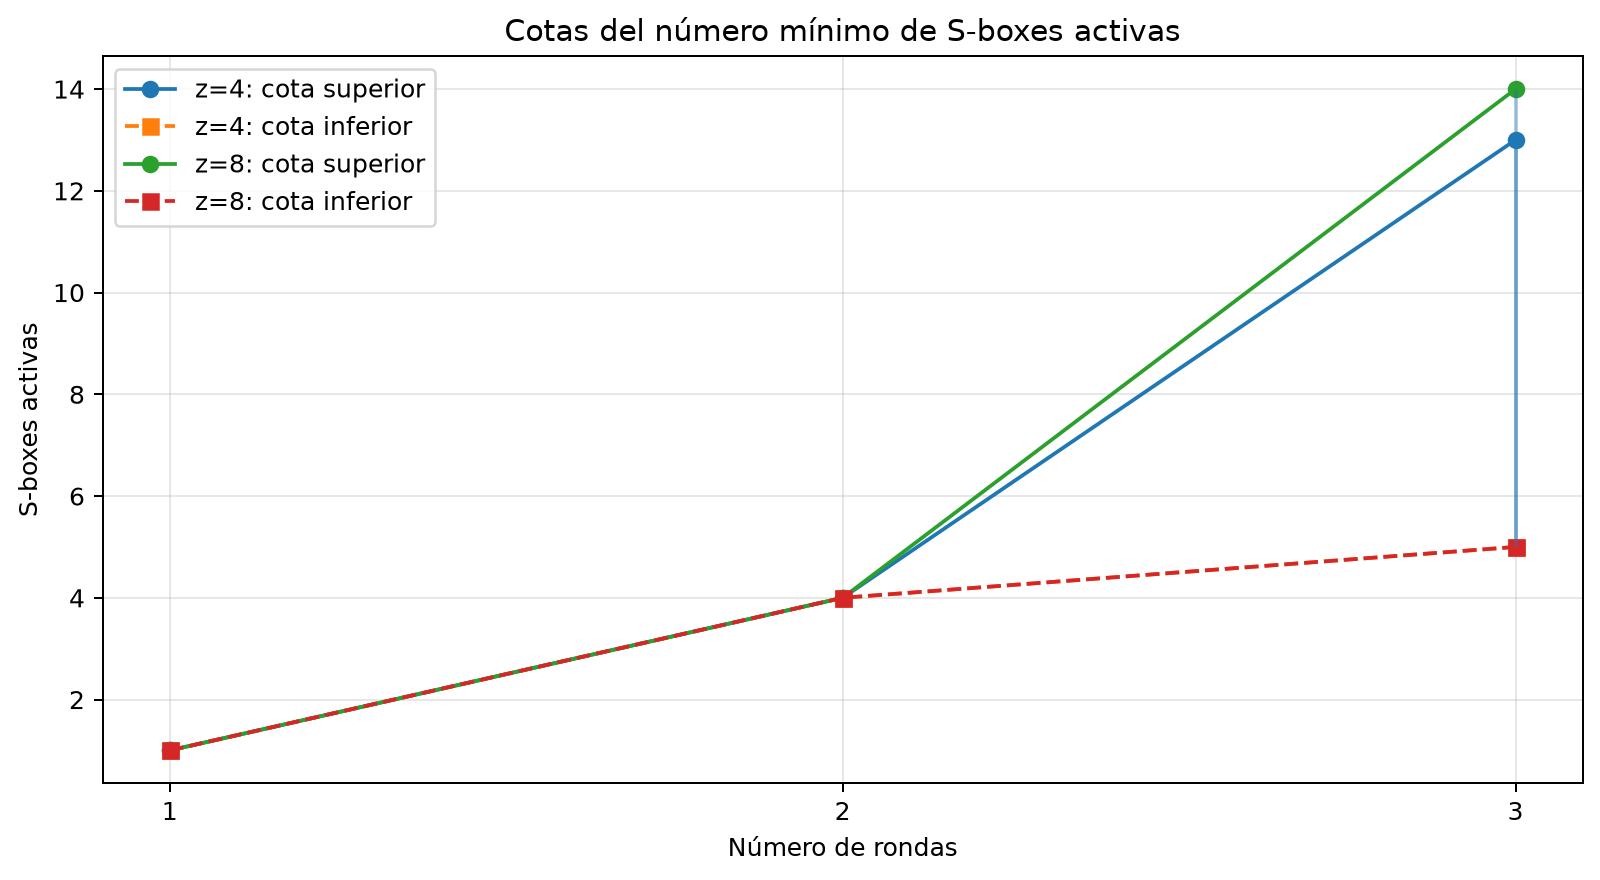
\includegraphics[
        width=0.85\textwidth
    ]{../outputs/figures/active_sbox_bounds.png}
    \caption{Cotas inferiores y superiores del número de S-boxes activas
    para $z=4$ y $z=8$.}
    \label{fig:cotas_sboxes}
\end{figure}

En una y dos rondas, la cota inferior coincide con la cota superior. Esta
coincidencia representa los mínimos globales certificados.

En tres rondas aparece una separación entre ambas cotas. Esta distancia
corresponde a la parte del problema que permanece abierta y no debe
confundirse con la brecha interna de optimalidad informada por CBC.


\subsection{Brecha de certificación}
\label{subsec:brecha_certificacion}

Para describir la amplitud del intervalo disponible se define la brecha de
certificación como

\[
G(z,R)
=
U(z,R)-L(z,R),
\]

donde $L(z,R)$ es la cota inferior global y $U(z,R)$ la actividad del mejor
testigo conocido.

Para tres rondas se obtiene

\[
G(4,3)
=
13-5
=
8,
\]

y

\[
G(8,3)
=
14-5
=
9.
\]

Esta medida expresa la distancia entre las evidencias matemáticas
disponibles. No corresponde a una brecha de optimalidad reportada por el
solver ni permite estimar en qué punto del intervalo se encuentra el
mínimo global.


\subsection{Comparación entre tamaños de palabra}
\label{subsec:comparacion_tamanos}

Los mínimos globales de una y dos rondas son iguales para los dos tamaños
de palabra:

\[
N_{\mathrm{act}}^{\min}(4,1)
=
N_{\mathrm{act}}^{\min}(8,1),
\]

\[
N_{\mathrm{act}}^{\min}(4,2)
=
N_{\mathrm{act}}^{\min}(8,2).
\]

Esta igualdad indica que, para los horizontes estudiados, duplicar la
longitud de palabra y el número de aplicaciones locales de $\chi$ por
ronda no obliga a incrementar el mínimo global.

En tres rondas, los mejores testigos restringidos presentan una diferencia
de una S-box:

\[
13
\quad \text{para } z=4,
\]

frente a

\[
14
\quad \text{para } z=8.
\]

No obstante, esta diferencia no demuestra que el mínimo global aumente con
$z$. Las cotas inferiores permanecen iguales y los extremos superiores
provienen de una familia restringida. Por tanto, no puede establecerse una
relación general entre el tamaño de palabra y la actividad mínima de tres
rondas.


\subsection{Interpretación criptanalítica}
\label{subsec:interpretacion_criptanalitica}

Los resultados muestran tres comportamientos principales:

\begin{enumerate}
    \item \textbf{Localización en una ronda.}
    Una diferencia inicial no nula puede alcanzar una única aplicación
    local de $\chi$.

    \item \textbf{Difusión en dos rondas.}
    La interacción entre las capas lineales y no lineales eleva el mínimo
    global a cuatro S-boxes activas.

    \item \textbf{Mayor dispersión en tres rondas.}
    Las mejores extensiones encontradas dentro de la familia $2+2+c$
    activan nueve o diez S-boxes adicionales en la tercera ronda.
\end{enumerate}

El conteo de S-boxes activas mide cuántos componentes no lineales reciben
una diferencia, pero no determina la probabilidad completa de una
característica diferencial. Dos trayectorias con la misma actividad pueden
presentar diferentes transiciones locales y, por tanto, probabilidades
distintas.

Para obtener una evaluación diferencial más completa sería necesario
incorporar los pesos de las transiciones de $\chi$ y analizar su
compatibilidad a lo largo de las rondas. En el alcance de este trabajo,
la actividad se interpreta como una medida estructural de difusión no
lineal.


\subsection{Síntesis de los resultados}
\label{subsec:sintesis_resultados}

Los seis experimentos pueden resumirse mediante

\[
N_{\mathrm{act}}^{\min}(4,1)=1,
\qquad
N_{\mathrm{act}}^{\min}(4,2)=4,
\qquad
5
\leq
N_{\mathrm{act}}^{\min}(4,3)
\leq
13,
\]

y

\[
N_{\mathrm{act}}^{\min}(8,1)=1,
\qquad
N_{\mathrm{act}}^{\min}(8,2)=4,
\qquad
5
\leq
N_{\mathrm{act}}^{\min}(8,3)
\leq
14.
\]

Los resultados de una y dos rondas son mínimos globales. Los resultados de
tres rondas son intervalos formados por una cota inferior global y una cota
superior respaldada por un testigo concreto.

Los valores 13 y 14 son óptimos dentro de la familia $2+2+c$, pero no se
presentan como mínimos globales del espacio completo de tres rondas.
\section{Validación y reproducibilidad}
\label{sec:reproducibilidad}

Los resultados se acompañan de una cadena de validación que incluye una
implementación funcional independiente, pruebas automatizadas, testigos
reconstruibles, archivos estructurados y versiones identificables mediante
Git.

El propósito de esta sección es describir los elementos necesarios para
verificar las afirmaciones principales del trabajo sin repetir los detalles
de arquitectura presentados en la
Sección~\ref{sec:arquitectura_implementacion}.


\subsection{Entorno computacional}
\label{subsec:entorno_computacional}

La implementación se desarrolló en el entorno resumido en la
Tabla~\ref{tab:entorno_computacional}.

\begin{table}[htbp]
    \centering
    \caption{Entorno utilizado en los experimentos.}
    \label{tab:entorno_computacional}
    \begin{tabular}{p{0.30\textwidth}p{0.60\textwidth}}
        \hline
        \textbf{Componente} & \textbf{Configuración} \\
        \hline
        Sistema operativo & Microsoft Windows 10 \\
        Lenguaje & Python 3.12.10 \\
        Modelado matemático & PuLP \\
        Solver & CBC mediante la interfaz de PuLP \\
        Control de versiones & Git y GitHub \\
        Informe & \LaTeX, \texttt{biblatex} y Biber \\
        \hline
    \end{tabular}
\end{table}

La información específica de cada ejecución se almacena en

\begin{center}
\texttt{outputs/results/experiment\_environment.json}.
\end{center}

Este archivo registra las versiones disponibles, el modo de ejecución y
los datos de trazabilidad del experimento. Los tiempos observados se
consideran referencias operativas y pueden variar según el equipo, la
versión del solver y la carga del sistema.


\subsection{Procedimiento de reproducción}
\label{subsec:procedimiento_reproduccion}

Desde la raíz del repositorio, la reproducción mínima requiere ejecutar
la suite de pruebas y regenerar los artefactos experimentales:

\begin{verbatim}
python -m pytest -q --disable-warnings
python scripts/run_active_sbox_experiments.py --mode quick
\end{verbatim}

El modo \texttt{quick} utiliza los resultados permanentes de las búsquedas
más costosas y regenera:

\begin{itemize}
    \item la tabla consolidada de experimentos;
    \item los testigos almacenados;
    \item el resumen de resultados;
    \item la información del entorno;
    \item la figura comparativa de cotas.
\end{itemize}

Para repetir desde cero la búsqueda restringida de tres rondas se utiliza:

\begin{verbatim}
python scripts/run_active_sbox_experiments.py --mode full
\end{verbatim}

Este modo vuelve a evaluar las trayectorias de la familia

\[
2+2+c
\]

para $z=4$ y $z=8$.

El informe se compila desde la carpeta \texttt{report/} mediante:

\begin{verbatim}
latexmk -pdf -interaction=nonstopmode -halt-on-error main.tex
\end{verbatim}

Si la bibliografía se gestiona mediante Biber, \texttt{latexmk} ejecuta
automáticamente las etapas necesarias siempre que el archivo
\texttt{.bcf} se haya generado correctamente.


\subsection{Pruebas automatizadas}
\label{subsec:pruebas_automatizadas}

La suite global de la versión utilizada en el informe alcanzó

\[
245
\]

pruebas aprobadas.

Las pruebas cubren los siguientes aspectos:

\begin{itemize}
    \item transformaciones individuales de Keccak reducido;
    \item composición de rondas completas;
    \item restricciones XOR y productos binarios;
    \item correspondencia entre la implementación funcional y el modelo
    MILP;
    \item cálculo de diferencias y soportes activos;
    \item restricciones de actividad total y actividad por ronda;
    \item búsqueda restringida de trayectorias $2+2+c$;
    \item reconstrucción de testigos;
    \item generación y lectura de los artefactos experimentales.
\end{itemize}

La aprobación de las pruebas reduce el riesgo de errores de implementación,
pero no constituye una demostración formal de corrección completa del
software.

Durante la ejecución pueden aparecer advertencias de PuLP relacionadas con
interfaces marcadas para futura obsolescencia. Estas advertencias no
corresponden a fallos de factibilidad, optimalidad o reconstrucción de los
resultados.


\subsection{Reconstrucción de testigos}
\label{subsec:reconstruccion_testigos}

Cada testigo utilizado en los resultados contiene información suficiente
para recuperar los estados iniciales

\[
A_0^L
\qquad \text{y} \qquad
A_0^R.
\]

A partir de estos estados se ejecutan nuevamente las rondas mediante la
implementación funcional. Para cada ronda se calcula

\[
\Delta B_r
=
B_r^L \oplus B_r^R
\]

y se reconstruye el soporte activo

\[
S_r
=
\left\{
(y,k):
\bigvee_{x=0}^{4}
\Delta B_r[x,y,k]=1
\right\}.
\]

La actividad por ronda se obtiene como

\[
m_r=|S_r|.
\]

Un testigo se considera validado cuando se cumplen simultáneamente las
siguientes condiciones:

\begin{enumerate}
    \item los estados intermedios coinciden con las transformaciones de
    referencia;

    \item las diferencias almacenadas coinciden con los XOR reconstruidos;

    \item los soportes activos coinciden con las posiciones no nulas de
    $\Delta B_r$;

    \item la suma

    \[
    \sum_{r=0}^{R-1}m_r
    \]

    coincide con la actividad total reportada;

    \item los estados y soportes son consistentes con las restricciones del
    modelo MILP.
\end{enumerate}

Esta reconstrucción permite verificar independientemente los resultados
exactos de una y dos rondas y los testigos utilizados como cotas superiores
en tres rondas.


\subsection{Artefactos experimentales}
\label{subsec:artefactos_experimentales}

Los resultados se almacenan en archivos estructurados para evitar la
transcripción manual de valores. La
Tabla~\ref{tab:artefactos_experimentales} resume los artefactos principales.

\begin{table}[htbp]
    \centering
    \caption{Artefactos principales para reproducción y auditoría.}
    \label{tab:artefactos_experimentales}
    \begin{tabular}{p{0.42\textwidth}p{0.50\textwidth}}
        \hline
        \textbf{Artefacto} & \textbf{Contenido} \\
        \hline

        \texttt{active\_sbox\_results.csv}
        &
        Cotas, actividades y clasificación de los seis experimentos.
        \\[3pt]

        \texttt{active\_sbox\_witnesses.json}
        &
        Estados, diferencias y soportes necesarios para reconstruir los
        testigos.
        \\[3pt]

        \texttt{active\_sbox\_summary.md}
        &
        Resumen legible de los resultados principales.
        \\[3pt]

        \texttt{experiment\_environment.json}
        &
        Versiones, modo de ejecución y datos del entorno.
        \\[3pt]

        \texttt{active\_sbox\_bounds.png}
        &
        Comparación gráfica de las cotas inferiores y superiores.
        \\[3pt]

        \texttt{keccak\_milp\_active\_sboxes.ipynb}
        &
        Notebook ejecutable con tablas, figura y comprobaciones dirigidas.
        \\
        \hline
    \end{tabular}
\end{table}

Los archivos de resultados se encuentran dentro de
\texttt{outputs/results/}, la figura dentro de
\texttt{outputs/figures/} y el notebook dentro de
\texttt{notebooks/}.

La separación entre resultados numéricos, testigos y datos del entorno
facilita la auditoría y permite reutilizar los artefactos desde otros
scripts.


\subsection{Validación del notebook}
\label{subsec:validacion_notebook}

El notebook final fue ejecutado completamente antes de generar la versión
utilizada en el informe. La revisión comprobó que:

\begin{itemize}
    \item no existieran errores almacenados;
    \item todas las celdas de código hubieran sido ejecutadas;
    \item estuvieran incluidos los resultados para $z=4$ y $z=8$;
    \item aparecieran los testigos de tres rondas;
    \item las tablas y la figura coincidieran con los archivos generados
    por el ejecutor experimental.
\end{itemize}

El notebook funciona como una interfaz de inspección de los resultados,
pero los valores principales provienen de los archivos estructurados
generados por los scripts del proyecto.


\subsection{Trazabilidad mediante Git}
\label{subsec:trazabilidad_git}

La versión experimental utilizada en este informe se identifica mediante:

\begin{itemize}
    \item repositorio:

    \begin{center}
    \url{https://github.com/hsancheza90-art/keccak-milp-criptografia}
    \end{center}

    \item etiqueta:

    \begin{center}
    \texttt{keccak-milp-experiments-v1}
    \end{center}

    \item commit:

    \begin{center}
    \texttt{0b089aa}
    \end{center}
\end{itemize}

La etiqueta identifica un estado estable del proyecto y permite separar los
resultados utilizados en el informe de cambios posteriores realizados en la
rama de desarrollo.


\subsection{Alcance de la reproducibilidad}
\label{subsec:alcance_reproducibilidad}

El modo rápido permite regenerar los resultados permanentes y verificar la
cadena completa de archivos sin repetir las enumeraciones de mayor costo.
El modo completo vuelve a ejecutar la búsqueda restringida de tres rondas.

En ambos casos pueden verificarse:

\begin{itemize}
    \item los mínimos globales de una ronda;
    \item los mínimos globales de dos rondas;
    \item las cotas inferiores de tres rondas;
    \item los testigos $2+2+9$ y $2+2+10$;
    \item la consistencia entre los archivos, el notebook y el informe.
\end{itemize}

La reproducibilidad no implica que los tiempos de ejecución sean idénticos
en todos los equipos. Tampoco convierte los testigos de tres rondas en
óptimos globales. Su propósito es garantizar que las afirmaciones puedan
ser reconstruidas y contrastadas a partir del código y de los artefactos
publicados.
\section{Limitaciones y amenazas a la validez}
\label{sec:limitaciones}

Los resultados deben interpretarse dentro del alcance del modelo, de las
configuraciones reducidas analizadas y del nivel de certificación alcanzado
en cada experimento. Esta sección resume las principales limitaciones
criptográficas, matemáticas y computacionales del trabajo.


\subsection{Alcance de las configuraciones reducidas}
\label{subsec:alcance_configuraciones_reducidas}

El estudio considera tamaños de palabra

\[
z \in \{4,8\},
\]

correspondientes a estados de 100 y 200 bits. Estas configuraciones
conservan la organización tridimensional de Keccak y la secuencia de
transformaciones

\[
\theta,
\quad
\rho,
\quad
\pi,
\quad
\chi,
\quad
\iota,
\]

pero no corresponden a la instancia Keccak-$f[1600]$ utilizada por SHA-3.

Por tanto, los resultados no deben interpretarse como una evaluación
directa de la seguridad de SHA-3 ni como mínimos aplicables
automáticamente a tamaños de palabra mayores. Su finalidad es estudiar la
formulación MILP y la propagación de diferencias en configuraciones
computacionalmente manejables.

De forma similar, el análisis se limita a un máximo de tres rondas. El
crecimiento de las variables binarias, las restricciones auxiliares y el
espacio de ramificación dificulta extender directamente la formulación a
más rondas mediante CBC.


\subsection{Alcance de la métrica de actividad}
\label{subsec:alcance_metrica_actividad}

La variable principal es el número de aplicaciones locales de $\chi$ que
reciben una diferencia de entrada no nula. Esta medida permite cuantificar
la cantidad de componentes no lineales atravesados por una trayectoria,
pero no representa por sí sola su probabilidad diferencial.

Dos trayectorias con el mismo número de S-boxes activas pueden contener
transiciones locales diferentes y, en consecuencia, presentar
probabilidades distintas. El modelo tampoco calcula directamente:

\begin{itemize}
    \item el peso diferencial de cada transición de $\chi$;
    \item la probabilidad acumulada de una trayectoria;
    \item el número de características compatibles con un mismo soporte;
    \item correlaciones lineales;
    \item la complejidad de un ataque contra SHA-3.
\end{itemize}

En consecuencia, la minimización de actividad identifica trayectorias
estructuralmente poco dispersas, pero no garantiza que sean las
trayectorias diferenciales más probables.

Una extensión natural consistiría en incorporar pesos asociados a las
transiciones diferenciales de $\chi$ y minimizar el peso total, en lugar
de utilizar únicamente indicadores binarios de actividad.


\subsection{Brecha de certificación en tres rondas}
\label{subsec:limitacion_tres_rondas}

El nivel de certificación no es igual para todos los experimentos.

Para una y dos rondas se obtuvo una coincidencia entre las cotas inferiores
y los testigos factibles. Por tanto, los valores reportados corresponden a
mínimos globales.

Para tres rondas solo se dispone de los intervalos

\[
5
\leq
N_{\mathrm{act}}^{\min}(4,3)
\leq
13,
\]

y

\[
5
\leq
N_{\mathrm{act}}^{\min}(8,3)
\leq
14.
\]

Las cotas inferiores son globales y los extremos superiores están
respaldados por testigos concretos. Sin embargo, no se demostró que no
existan trayectorias con actividades comprendidas dentro de estos
intervalos.

Por esta razón, los valores 13 y 14 no constituyen mínimos globales
certificados.


\subsubsection{Restricción de la familia \texorpdfstring{$2+2+c$}{2+2+c}}

La búsqueda de tres rondas se restringió a trayectorias cuya actividad en
las dos primeras rondas es

\[
2+2.
\]

Dentro de esta familia, la enumeración fue exhaustiva y produjo los mejores
valores

\[
2+2+9=13
\]

para $z=4$, y

\[
2+2+10=14
\]

para $z=8$.

No obstante, una trayectoria globalmente mejor podría presentar una
distribución diferente, por ejemplo,

\[
1+a+b,
\qquad
3+a+b,
\qquad
m_0+m_1+m_2,
\]

siempre que satisfaga las restricciones exactas de propagación.

En consecuencia, la afirmación correcta es:

\begin{quote}
La búsqueda es exhaustiva dentro de la familia $2+2+c$, pero no dentro
del espacio completo de trayectorias de tres rondas.
\end{quote}

Cerrar los intervalos requeriría explorar otras distribuciones de actividad,
fortalecer la formulación MILP o emplear métodos de descomposición más
generales.


\subsection{Dependencia del solver y del entorno}
\label{subsec:dependencia_solver_entorno}

CBC permitió resolver los casos de una y dos rondas, validar testigos y
demostrar la infactibilidad de determinados problemas auxiliares. Sin
embargo, su capacidad de certificación disminuye al aumentar el tamaño del
modelo.

El crecimiento de $z$ y $R$ incrementa:

\begin{itemize}
    \item las variables de los estados izquierdo y derecho;
    \item las variables de diferencia;
    \item las variables auxiliares para XOR y productos;
    \item las restricciones de cada transformación;
    \item el espacio explorado mediante ramificación y acotación.
\end{itemize}

Una terminación por límite de tiempo no demuestra que el modelo sea
infactible ni que la mejor solución encontrada sea óptima. En este trabajo
solo se utilizan como certificadas las conclusiones respaldadas por un
estado concluyente del solver o por un testigo reconstruido
independientemente.

El uso de un solver comercial, como Gurobi, podría reducir los tiempos de
resolución mediante mejores procedimientos de \emph{presolve}, cortes,
heurísticas y paralelización. No obstante, un solver más rápido no elimina
la necesidad de distinguir entre:

\begin{itemize}
    \item una solución factible;
    \item una cota inferior;
    \item una prueba de infactibilidad;
    \item una prueba de optimalidad global.
\end{itemize}

Los tiempos de ejecución también dependen del procesador, la memoria, las
versiones de Python, PuLP y CBC, y la carga concurrente del sistema. Por
ello, se reportan como referencias de reproducibilidad y no como una
comparación formal de rendimiento.


\subsection{Validez de la implementación}
\label{subsec:validez_implementacion}

La validez interna se fortalece mediante:

\begin{itemize}
    \item una implementación funcional independiente;
    \item comparación bit a bit entre la referencia y el modelo MILP;
    \item reconstrucción de estados, diferencias y soportes;
    \item generación automática de resultados;
    \item pruebas unitarias y de integración;
    \item control de versiones y testigos almacenados.
\end{itemize}

Estas medidas reducen el riesgo de aceptar resultados producidos por
errores de programación o de extracción de variables. Sin embargo, como en
cualquier implementación computacional, las pruebas automatizadas no
constituyen una demostración formal de la corrección total del software.

Los testigos almacenados demuestran la existencia de trayectorias con una
actividad determinada, pero no describen todas las soluciones con el mismo
valor. Pueden existir diferentes soportes, estados absolutos o soluciones
relacionadas mediante simetrías que produzcan la misma actividad.

Por tanto, los testigos deben interpretarse como certificados de
factibilidad y no como representantes únicos de todas las trayectorias
óptimas o cuasi-óptimas.


\subsection{Correspondencia entre intentos y rondas}
\label{subsec:limitacion_intentos_rondas}

La relación

\[
R(t)=
\begin{cases}
1, & t<10,\\
2, & 10\leq t<20,\\
3, & 20\leq t<30
\end{cases}
\]

se incorporó para responder al planteamiento de la actividad académica.

Esta relación no pertenece a la definición de Keccak y no representa una
conexión criptográfica demostrada entre el número de intentos de un
atacante y el número de rondas de la permutación. En la implementación,
los intentos funcionan únicamente como un parámetro externo para seleccionar
uno de los tres escenarios experimentales.

Por esta razón, las conclusiones se expresan principalmente en términos de
$z$ y $R$, y no como una relación general entre intentos y seguridad.


\subsection{Síntesis de las amenazas a la validez}
\label{subsec:sintesis_amenazas}

La Tabla~\ref{tab:amenazas_validez} resume las principales amenazas y las
medidas adoptadas para reducirlas.

\begin{table}[htbp]
    \centering
    \caption{Principales amenazas a la validez y medidas de mitigación.}
    \label{tab:amenazas_validez}
    \begin{tabular}{
        p{0.24\textwidth}
        p{0.31\textwidth}
        p{0.35\textwidth}
    }
        \hline
        \textbf{Amenaza}
        &
        \textbf{Consecuencia}
        &
        \textbf{Mitigación}
        \\
        \hline

        Tamaños y rondas reducidos
        &
        Los resultados no se trasladan automáticamente a Keccak-$f[1600]$.
        &
        Delimitación explícita del alcance y uso de configuraciones
        estructuralmente válidas.
        \\[4pt]

        Métrica basada en actividad
        &
        No se obtiene la probabilidad diferencial completa.
        &
        Interpretación estructural y propuesta de incorporar pesos
        diferenciales.
        \\[4pt]

        Brecha en tres rondas
        &
        No se conoce el mínimo global exacto.
        &
        Reporte mediante intervalos y distinción entre cotas y óptimos.
        \\[4pt]

        Búsqueda $2+2+c$
        &
        Pueden existir mejores distribuciones fuera de la familia.
        &
        Declaración explícita de la restricción y conservación de los
        testigos como cotas superiores globales.
        \\[4pt]

        Dependencia del solver
        &
        Los tiempos y la capacidad de certificación pueden variar.
        &
        Uso exclusivo de estados certificados y validación independiente.
        \\[4pt]

        Errores de implementación
        &
        Una formulación incorrecta podría producir resultados inválidos.
        &
        Implementación de referencia, pruebas automatizadas y
        reconstrucción de testigos.
        \\
        \hline
    \end{tabular}
\end{table}

Estas limitaciones no invalidan los resultados obtenidos. Definen el
contexto dentro del cual pueden considerarse correctos y evitan extender
las conclusiones más allá de la evidencia disponible.
\section{Conclusiones}
\label{sec:conclusiones}

Este trabajo desarrolló un modelo de Programación Lineal Entera Mixta para
estudiar el número mínimo de aplicaciones activas de la capa no lineal
$\chi$ en versiones reducidas de Keccak.

La formulación representa bit a bit dos ejecuciones simultáneas de la
permutación y calcula sus diferencias mediante restricciones XOR exactas.
Las transformaciones $\theta$, $\rho$, $\pi$, $\chi$ e $\iota$ se modelaron
de acuerdo con la estructura de una ronda de Keccak, mientras que las
variables binarias $a_{r,y,k}$ permitieron identificar y minimizar la
actividad de cada aplicación local de $\chi$.

El modelo se aplicó a tamaños de palabra

\[
z\in\{4,8\},
\]

correspondientes a estados de 100 y 200 bits y a 20 y 40 aplicaciones
locales de $\chi$ por ronda, respectivamente. Los experimentos consideraron
una, dos y tres rondas.


\subsection{Respuesta al objetivo del trabajo}
\label{subsec:respuesta_objetivo}

El objetivo principal consistía en modelar Keccak reducido mediante MILP
y determinar o acotar el número mínimo de S-boxes activas para diferentes
tamaños de palabra y números de rondas.

La implementación desarrollada responde a este objetivo mediante:

\begin{itemize}
    \item una representación exacta de las transformaciones de Keccak;
    \item dos ejecuciones simultáneas para calcular diferencias XOR;
    \item variables binarias para identificar las S-boxes activas;
    \item una función objetivo que minimiza la actividad total;
    \item problemas auxiliares de factibilidad para establecer cotas;
    \item testigos concretos reconstruibles mediante una implementación
    funcional independiente.
\end{itemize}

La correspondencia entre intentos y rondas se utilizó únicamente como
criterio experimental. No se interpretó como una modificación interna de
Keccak ni como una relación criptográfica demostrada entre intentos de un
atacante y profundidad de la permutación.


\subsection{Resultados principales}
\label{subsec:conclusiones_resultados}

Para una ronda se certificó

\[
N_{\mathrm{act}}^{\min}(4,1)
=
N_{\mathrm{act}}^{\min}(8,1)
=
1.
\]

La cota inferior se deriva de la imposibilidad de que una diferencia no
nula desaparezca después de las transformaciones lineales. La existencia
de testigos con una sola S-box activa completa la prueba de optimalidad
global.

Para dos rondas se obtuvo

\[
N_{\mathrm{act}}^{\min}(4,2)
=
N_{\mathrm{act}}^{\min}(8,2)
=
4.
\]

CBC demostró que no existe una trayectoria con actividad total menor o
igual que tres, mientras que los testigos reconstruidos alcanzaron la
distribución

\[
2+2.
\]

La coincidencia entre ambas evidencias permite afirmar que cuatro es el
mínimo global para los dos tamaños de palabra.

Para tres rondas se establecieron los intervalos

\[
5
\leq
N_{\mathrm{act}}^{\min}(4,3)
\leq
13,
\]

y

\[
5
\leq
N_{\mathrm{act}}^{\min}(8,3)
\leq
14.
\]

Las cotas inferiores son globales y se derivan del mínimo exacto de dos
rondas junto con la necesidad de activar al menos una S-box adicional en
la tercera ronda.

Las cotas superiores están respaldadas por testigos con distribuciones

\[
2+2+9
\]

para $z=4$, y

\[
2+2+10
\]

para $z=8$.

Los valores 13 y 14 son óptimos dentro de la familia restringida
$2+2+c$, pero no constituyen mínimos globales certificados para el espacio
completo de tres rondas.


\subsection{Interpretación}
\label{subsec:conclusiones_interpretacion}

Los resultados muestran que una diferencia puede permanecer localizada
durante una ronda, pero la difusión acumulada incrementa la cantidad mínima
de componentes no lineales activos cuando se consideran más rondas.

La igualdad de los mínimos para $z=4$ y $z=8$ en una y dos rondas indica
que duplicar el tamaño de palabra y el número de aplicaciones locales de
$\chi$ no obliga, en estos horizontes, a aumentar la actividad mínima.

En tres rondas, los mejores testigos restringidos difieren en una S-box.
Sin embargo, como las cotas inferiores son iguales y los extremos superiores
provienen de una familia específica, no puede concluirse que el mínimo
global aumente necesariamente con el tamaño de palabra.

El número de S-boxes activas debe interpretarse como una medida estructural
de propagación no lineal. Esta cantidad no determina por sí sola la
probabilidad diferencial de una trayectoria ni la seguridad completa de
SHA-3.


\subsection{Aporte metodológico y computacional}
\label{subsec:aporte_metodologico}

La principal ventaja de la formulación pareada es que la propagación a
través de $\chi$ surge de dos evaluaciones exactas de la función booleana.
Esto evita depender exclusivamente de una aproximación diferencial
truncada y permite recuperar parejas concretas de estados.

CBC fue suficiente para:

\begin{itemize}
    \item obtener y validar testigos;
    \item demostrar infactibilidad en problemas auxiliares;
    \item certificar los mínimos globales de una y dos rondas;
    \item verificar estados y soportes obtenidos mediante enumeración.
\end{itemize}

Para tres rondas fue necesario complementar el modelo MILP con una búsqueda
exhaustiva restringida. Esta combinación permitió obtener testigos
verificables sin atribuirles un nivel de optimalidad superior al respaldado
por las evidencias.

La implementación se acompañó de una referencia funcional independiente,
artefactos estructurados y una suite de 245 pruebas automatizadas. Estos
elementos fortalecen la trazabilidad y permiten reconstruir los resultados
principales.


\subsection{Limitación principal}
\label{subsec:conclusion_limitacion}

La principal limitación es que el mínimo global de tres rondas permanece
abierto.

La búsqueda realizada es exhaustiva dentro de la familia

\[
2+2+c,
\]

pero no considera todas las distribuciones posibles de actividad durante
las tres rondas. En consecuencia, el resultado correcto para estos
experimentos es un intervalo de certificación y no un único valor exacto.

Esta distinción es esencial: los testigos de actividades 13 y 14 demuestran
que existen trayectorias con dichos valores, pero no descartan la existencia
de trayectorias globalmente mejores.


\subsection{Trabajo futuro}
\label{subsec:trabajo_futuro}

Las extensiones más relevantes del trabajo son:

\begin{enumerate}
    \item explorar distribuciones de tres rondas diferentes de
    $2+2+c$;

    \item incorporar restricciones de ruptura de simetrías y desigualdades
    válidas que fortalezcan la relajación del modelo;

    \item comparar CBC con solvers de mayor rendimiento, como Gurobi;

    \item desarrollar estrategias de descomposición que separen la
    generación de soportes, la asignación de valores absolutos y la
    validación MILP;

    \item incorporar pesos diferenciales de $\chi$ para minimizar el peso
    de una trayectoria y no únicamente el número de S-boxes activas;

    \item evaluar tamaños de palabra y números de rondas mayores.
\end{enumerate}


\subsection{Conclusión final}
\label{subsec:conclusion_final}

El número mínimo de S-boxes activas en Keccak reducido puede estudiarse de
manera sistemática mediante una combinación de modelado MILP, problemas de
factibilidad, enumeración controlada y validación independiente.

Para una y dos rondas se obtuvieron mínimos globales exactos. Para tres
rondas se construyeron cotas globales y testigos reproducibles, manteniendo
una distinción explícita entre optimalidad global y optimalidad restringida.

En conjunto, la implementación proporciona una respuesta rigurosa a la
actividad planteada y establece una base extensible para futuros estudios
de propagación diferencial en Keccak.


\section*{Disponibilidad del código y los artefactos}
\addcontentsline{toc}{section}{Disponibilidad del código y los artefactos}
\label{sec:disponibilidad_codigo}

El código fuente, las pruebas automatizadas, el notebook y los artefactos
experimentales se encuentran disponibles en:

\begin{center}
\url{https://github.com/hsancheza90-art/keccak-milp-criptografia}
\end{center}

La versión utilizada para los resultados del informe está identificada
mediante:

\begin{center}
\texttt{keccak-milp-experiments-v1}
\end{center}

y el commit:

\begin{center}
\texttt{0b089aa}.
\end{center}

Los comandos de reproducción, la descripción de los archivos generados y
el procedimiento de validación se presentan en la
Sección~\ref{sec:reproducibilidad}.
\section*{Disponibilidad del código y los artefactos}
\phantomsection
\label{sec:disponibilidad-codigo}

El código fuente, las pruebas automatizadas, los scripts de ejecución,
el notebook y los artefactos experimentales asociados con este trabajo
se encuentran disponibles públicamente en el repositorio:

\begin{center}
\url{https://github.com/hsancheza90-art/keccak-milp-criptografia}
\end{center}

Para garantizar la trazabilidad de los resultados, la versión utilizada
en este artículo se identifica mediante la etiqueta:

\begin{center}
\path{keccak-milp-experiments-v1}
\end{center}

La etiqueta corresponde al commit:

\begin{center}
\path{0b089aa}
\end{center}

La rama \path{feature/chi-milp} contiene el desarrollo del modelo y
puede recibir modificaciones posteriores. Por esta razón, la etiqueta
estable y el identificador del commit constituyen las referencias
recomendadas para reproducir los resultados presentados.

\subsection*{Estructura de los recursos publicados}

La Tabla~\ref{tab:published-resources} resume los recursos principales
del repositorio.

\begin{table}[H]
\centering
\caption{Recursos disponibles para reproducción y auditoría.}
\label{tab:published-resources}
\begin{tabularx}{\textwidth}{
    >{\raggedright\arraybackslash}p{0.40\textwidth}
    X
}
\toprule
\textbf{Recurso} & \textbf{Contenido} \\
\midrule

\path{src/keccak_milp/}
&
Implementación de referencia de Keccak reducido, formulación MILP,
modelo diferencial pareado y funciones de búsqueda.
\\

\path{scripts/run_active_sbox_experiments.py}
&
Punto de entrada para ejecutar la matriz de experimentos en los modos
\path{quick} y \path{full}.
\\

\path{tests/}
&
Pruebas unitarias, de integración, reconstrucción de testigos y
validación de artefactos.
\\

\path{notebooks/keccak_milp_active_sboxes.ipynb}
&
Notebook académico ejecutado, con tablas, figura, resultados,
interpretación y pruebas dirigidas.
\\

\path{outputs/results/active_sbox_results.csv}
&
Resultados consolidados de los seis experimentos.
\\

\path{outputs/results/active_sbox_witnesses.json}
&
Estados, soportes y datos necesarios para reconstruir los testigos.
\\

\path{outputs/results/experiment_environment.json}
&
Información del entorno y de la ejecución experimental.
\\

\path{outputs/figures/active_sbox_bounds.png}
&
Figura comparativa de las cotas inferiores y superiores.
\\

\path{report/}
&
Fuentes en LaTeX y versión compilable del artículo académico.
\\

\bottomrule
\end{tabularx}
\end{table}

\subsection*{Reproducción mínima}

Una reproducción funcional de los resultados permanentes puede
realizarse desde la raíz del repositorio mediante:

\begin{lstlisting}[language=bash]
python -m pytest -q --disable-warnings
python scripts/run_active_sbox_experiments.py --mode quick
\end{lstlisting}

Para volver a ejecutar las búsquedas exhaustivas restringidas de tres
rondas debe utilizarse:

\begin{lstlisting}[language=bash]
python scripts/run_active_sbox_experiments.py --mode full
\end{lstlisting}

El informe se compila desde la carpeta \path{report/}:

\begin{lstlisting}[language=bash]
latexmk -pdf -interaction=nonstopmode -halt-on-error main.tex
\end{lstlisting}

\subsection*{Referencia de la versión experimental}

La combinación de los siguientes elementos identifica de forma
unívoca la versión del trabajo utilizada en el artículo:

\begin{itemize}
    \item repositorio:
    \url{https://github.com/hsancheza90-art/keccak-milp-criptografia};

    \item etiqueta:
    \path{keccak-milp-experiments-v1};

    \item commit:
    \path{0b089aa};

    \item ejecutor:
    \path{scripts/run_active_sbox_experiments.py};

    \item notebook:
    \path{notebooks/keccak_milp_active_sboxes.ipynb}.
\end{itemize}

Esta información permite recuperar el código, verificar los testigos y
reconstruir las tablas y figuras sin depender de la evolución futura de
la rama de desarrollo.


% ============================================================
% Referencias
% ============================================================
\printbibliography[title={Referencias}]

\end{document}
